\chapter{Applied Modeling of Solid Breeders}\label{sec:dem-studies}

In the preceding chapters, descriptions of the microscale models established for this thesis were given. The new models were created to permit studying the internal packing structure of solid breeder pebble beds, specifically under fault conditions (\textit{i.e.} crushed pebbles, altered packing structures), and the subsequent ability to maintain heat removal of deposited nuclear energy. In this chapter we finally apply all the models toward studying heat transfer in fusion-relevant pebble bed configurations. There will be three main topics considered: (i) changes to effective conductivity due to irradiation damage of ceramic solids, (ii) the effect of pebble bed orientation, initial packing fraction, and pebble fragmentation on temperature distributions in pebble beds, and (iii) helium tortuosity effects on heat transfer after pebble fragmentation. 


\section{Irradiation Effects on Effective Thermal Conductivity}\label{sec:irradiation}
Ceramic materials primarily conduct heat by phonon transport. Irradiation-induced vacancies act as phonon scattering centers and consequently thermal conductivity of ceramics is reduced under irradiation.\cite{Hopkins1985} Fast neutron damage can produce large populations of defects and thereby reduce room-temperature thermal conductivity of ceramics by orders of magnitude with doses $\le 1$~dpa.\cite{Snead2005} Analysis of breeding blanket modules for ITER indicate a maximum expected neutron damage in steel to be about 3 dpa over a span of 20 years of operation. By comparison, dpa levels required for DEMO are greater than 70 dpa.\cite{Giancarli2006a} Reduced thermal conductivity due to fast neutron damage is a concern for blanket designers and this study is meant to address pebble bed thermal reactions to irradiated pebbles.

Neutron fluence in ITER is targeted to reach \SI{0.3}{\mega\watt\year\per\square\meter}.\cite{Abdou2015,VanHoutte2011} In terms of \SI{14}{\mega\electronvolt} neutrons, this equates to a fluence of \SI{4.22E24}{\neutron\per\meter\squared}. Kawamura\etal~carried out irradiation experiments on \lit~pebble beds to detect changes in effective thermal diffusivity. They found a reduction in thermal diffusivity of 30\% compared to unirradiated pebble beds at \SI{400}{\celsius} but report that no change in effective thermal conductivity is detectable up to thermal neutron fluence of \SI{1E24}{\neutron\per\meter\squared}. 

An experimental irradiation campaign has been carried out in Petten, Netherlands as part of the European program for development of HCPB blanket concept, a high fluence irradiation project, HICU (High neutron fluence Irradiation of pebble staCks for fUsion). The high fluence irradiation of lithium ceramics was meant to be up to DEMO-relevant values of 20 to 25 dpa, even with a neutron spectra not including \SI{14.1}{\mega\electronvolt}.\cite{Hegeman2003,VanTil2012} Temperatures in ceramic regions dropped during the experimental campaign, trailing somewhat the tritium production rate and lithium burn-up. On-line temperatures were measured during the year-long experiment, temperatures in ceramic pebble regions were measured between \SIrange{600}{800}{\kelvin}. Similar to Kawamura\etal, a significant increase in temperatures as a result of decreased thermal conductivity was not witnessed. However, careful thermal characterizations of ceramic pebble beds under irradiation were not evaluated.

The experiment of Kawamura\etal~reached neutron fluence of the same order of magnitude of a years operation in ITER though only with thermal neutrons. HICU matched much of the neutron energy spectrum, save for the highly energetic fusion neutrons. Both experiments did not detect significant reductions in thermal conductivity. The results are providential for ceramic breeder regions far from first walls. Nevertheless, damage from fast neutrons in near-wall regions remains a concern.

In this study, we investigate the effects on effective conductivity as impacted by two orders of magnitude reduction in solid conductivity. To simulate neutron damage of \lit~in solid breeder pebble beds, we will parametrically reduce the solid conductivity as $\eta = k_\text{irr} / k_\text{unirr}$, where $k_\text{irr}$ is a proxy value for the solid conductivity of material that has been damaged by neutron irradiation and $k_\text{unirr} = \SI{2.4}{\watt\per\meter\per\kelvin}$. In this study $\eta$ is varied from $\eta = 1$ down to $\eta = 0.01$ to cover a broad range of reduction. The nuclear heat generation rate is \SI{8}{\mega\watt\per\meter\cubed}. We calculate an effective thermal conductivity of pebble beds with damaged ceramics. The pebble bed geometries are duplicates of those used for validation in \Cref{sec:dem-benchmark}. The initial packing fraction of the pebble bed is $\phi_i = 0.61$. At thermal steady-state, temperature scatters of pebbles and binned average values are plotted for the neutron-damaged pebble beds in \Cref{fig:irrad-temps}. A $\keff$ is calculated for each bed and plotted alongside its fit in \Cref{fig:irrad-keff}; the effective thermal conductivity for irradiated beds is normalized against the case of non-irradiated bed, $\keff = \SI{0.398}{\watt\per\meter\per\kelvin}$. As a consequence of irradiation damage to conductivity, maximum temperatures in the pebble beds increased dramatically; average maximum values are plotted in \Cref{fig:irrad-mids}.

\begin{figure}[ht]
    \centering
    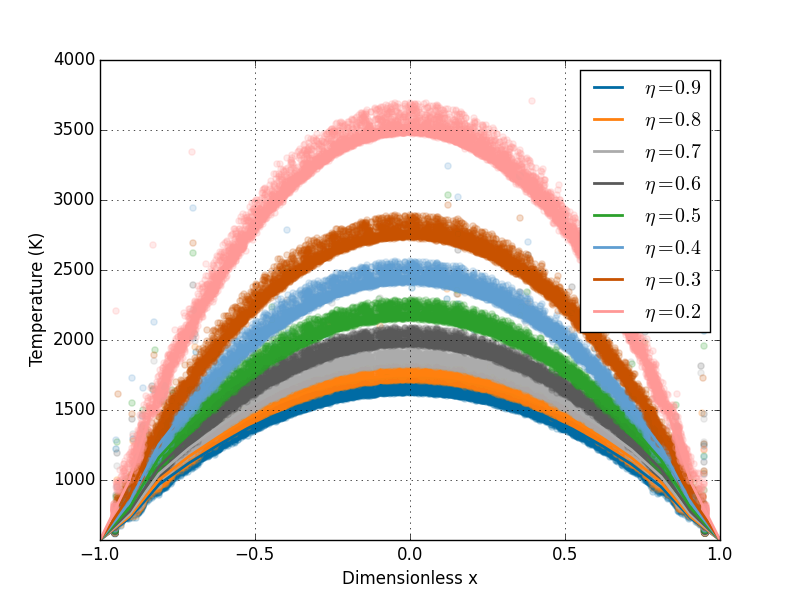
\includegraphics[width = 0.75\textwidth]{figures/irradiated/irradiated-temperatures.png}
    \caption{Temperature scatters and average profiles for DEM models of ceramic pebbles with irradiation-damage-induced reductions in thermal conductivity.}\label{fig:irrad-temps}
\end{figure}

\begin{figure}[ht]
    \centering
    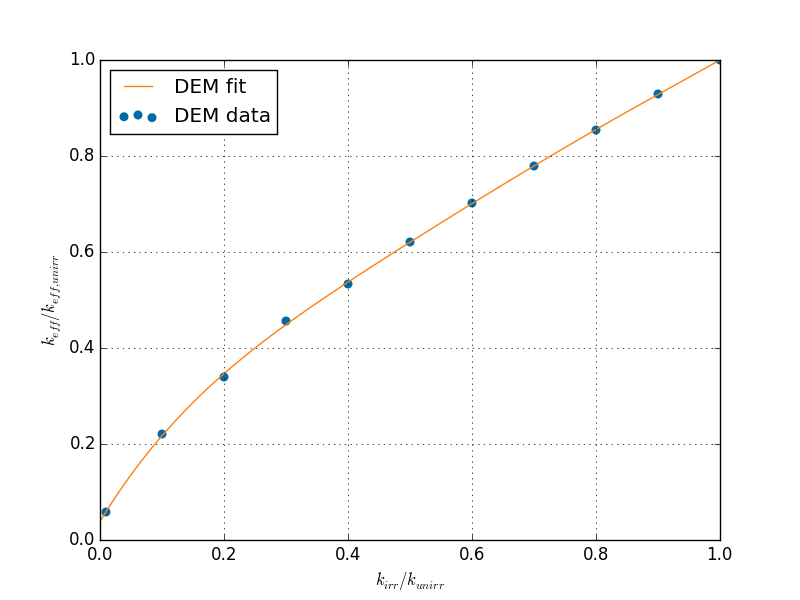
\includegraphics[width = 0.75\textwidth]{figures/irradiated/keff-plots.png}
    \caption{In DEM-based simulations, $\keff$ of pebble beds rapidly decreases as the solid conductivity drops by more than a single order of magnitude.}\label{fig:irrad-keff}
\end{figure}

\begin{figure}[ht]
    \centering
    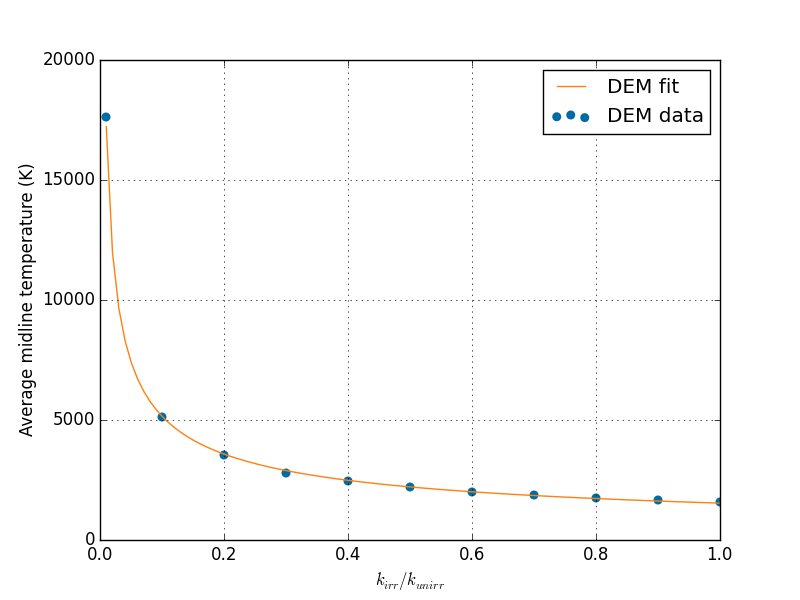
\includegraphics[width = 0.75\textwidth]{figures/irradiated/Tmid-plots.png}
    \caption{In DEM-based simulations, mid-line temperatures increase sharply as $\eta < 0.1$.}\label{fig:irrad-mids}
\end{figure}

The effective thermal conductivity is fit to the following fifth-order polynomial, with $R^2 = 0.9999$,
\begin{equation}
\keff [\si{\watt\per\meter\per\kelvin}] = 1.39 \eta^5 - 4.649 \eta^4 + 6.061 \eta^3 - 3.964 \eta^2 + 2.124 \eta + 0.03875
\end{equation}
Data for mid-line temperatures was fit to the following power law, with $R^2 = 0.9993$,
\begin{equation}
T_\text{mid}[\si{\kelvin}] = 1536.2\eta^{-0.526}
\end{equation}

In the DEM model, heat transport between constituents in pebble beds proceeds only through points of contact as if in vacuum. In the idealized situation considered here, as solid conductivity reduces due to neutron damage, $k_\text{irr} \rightarrow \SI{0}{\watt\per\meter\per\kelvin}$, the effective thermal conductivity must similarly converge to $\keff \rightarrow \SI{0}{\watt\per\meter\per\kelvin}$. The pebble temperatures of these beds will thereby increase to $T_p \rightarrow \infty$ because of the lack of the material to transport heat. This behavior is seen in \Cref{fig:irrad-keff} and \Cref{fig:irrad-temps}.

Bearing in mind that heat transfer in vacuum is not directly relevant to blanket operation but the results do facilitate observation of contact conductance's role in pebble bed heat transfer. For instance, when $\eta > 0.4$, reduction in irradiated $\keff$ is approximately linear with a slope of \num{0.77}. In other words, the effective thermal conductivity of beds of irradiated pebbles drops only 77\% of the reduction in solid conductivity of the irradiated pebbles themselves. Returning for a moment to \Cref{eq:cheng-modification-batchelor}, heat conductance between two pebbles is directly related to solid conductivity and radius of the contact area between them, $a$. However, there is not a one-to-one reduction in $H_c$ due to reductions in $k_s$. Nor is there an inflection point where the magnitude of $k_s$ decreases to be on the same order of magnitude, or less, than the contact radius; at an irradiated conductivity as low as $\eta = 0.01$, $k_{s,irr}$ is still, generally, three orders of magnitude larger than the contact radius, $a$. The reduction in $\keff$ for irradiated pebble beds, is instead due to combined effects of solid conductivity, coordination number, and contact forces. A thorough look into the relationship between heat transfer and parameters describing packing structures was reported by Van Lew\etal.\cite{VanLew2014}

The results in vacuum are interesting and illustrative, but not directly pertinent for blanket designers. Thus we now consider a more fusion-appropriate case of reduction in effective thermal conductivity due to neutron damage in the presence of helium. In this case, the pebble beds are re-creations of those from \Cref{sec:cfd-validate}, with packing fractions of $\phi_i = 0.62$ and stagnant helium. Again, pebble temperature scatter plots and binned average values are plotted for the neutron-damaged pebble beds in \Cref{fig:irrad-temps-cfd-q}, $\keff$ is given in \Cref{fig:irrad-keff-cfd-q}; the effective thermal conductivity for irradiated beds is normalized against the case of non-irradiated bed, $\keff = \SI{1.02}{\watt\per\meter\per\kelvin}$, average maximum values are plotted in \Cref{fig:irrad-mids-cfd-q}.

In the case of reduced solid conductivity, the Jeffreson correction to heat transfer coefficient becomes more pronounced. A sphere in a stagnant fluid has a Nusselt number of $\Nu = 2$, equating to a heat transfer coefficient of $h =\SI{680}{\watt\per\meter\squared\per\kelvin}$ for these pebbles in helium. The Biot number is a function of solid conductivity, $\Bi = hd_p/k_s$, inversely related to solid conductivity. The Biot number for irradiated pebbles is given in \Cref{fig:biot-changes}. Jeffreson correction accounts for large Biot numbers and reduces the heat transfer coefficient as $h_p = h/(1 + \Bi/5)$. Reduced heat transfer coefficients are also given in \Cref{fig:biot-changes}. The Biot number and heat transfer coefficients are normalized against the unirradiated condition. We see that, for example, when $\eta = 0.1$, meaning one order of magnitude reduction in solid conduction, the heat transfer coefficient reduces to 40\% of the original value. 

For the zero-velocity helium in this consideration, the fluid's volume-averaged energy equation at steady-state reduces to 
\begin{equation}
\nabla\left(\epsilon_k\nabla T_f\right) = \frac{1}{V_k\rho_fC_f}\sum_{\forall i \in k} h_i A_i \Delta T_{if}
\end{equation}
If an uncorrected heat transfer coefficient was introduced into this energy equation, the term on the right-hand-side would introduce large errors into the fluid temperature profile. Without the Jeffreson correction, the lumped capacitance assumption in the DEM framework would greatly over-estimate the amount of energy capable of being transported from pebble internals to fluid at the surface.

\begin{figure}[ht]
    \centering
    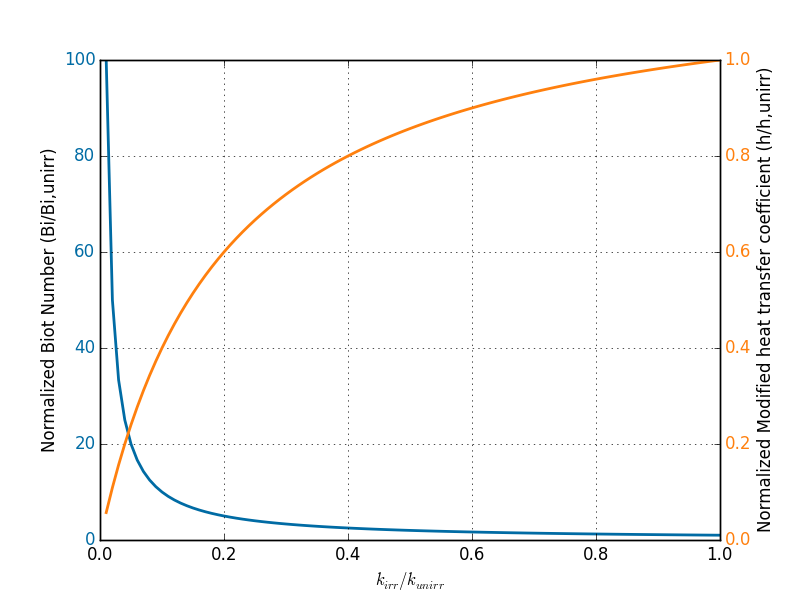
\includegraphics[width = 0.75\textwidth]{figures/irradiated/biot-changes.png}
    \caption{Biot number as a function of normalized solid conductivity (left), modified heat transfer coefficient \textit{via} Jeffreson correction (right).}\label{fig:biot-changes}
\end{figure}

\begin{figure}[ht]
    \centering
    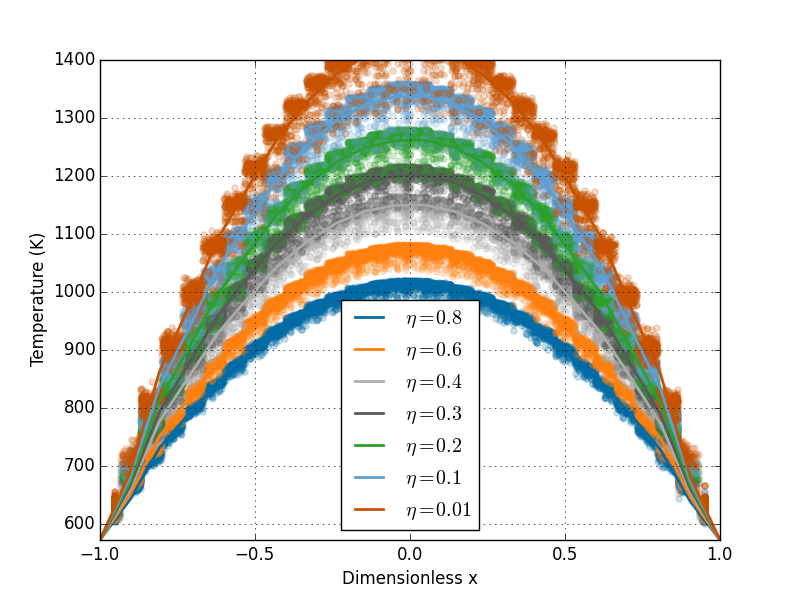
\includegraphics[width = 0.75\textwidth]{figures/irradiated/irradiated-temperatures-cfd-q.png}
    \caption{Temperature scatters and average profiles for CFD-DEM models of ceramic pebbles with irradiation-damage-induced reductions in thermal conductivity.}\label{fig:irrad-temps-cfd-q}
\end{figure}

\begin{figure}[ht]
    \centering
    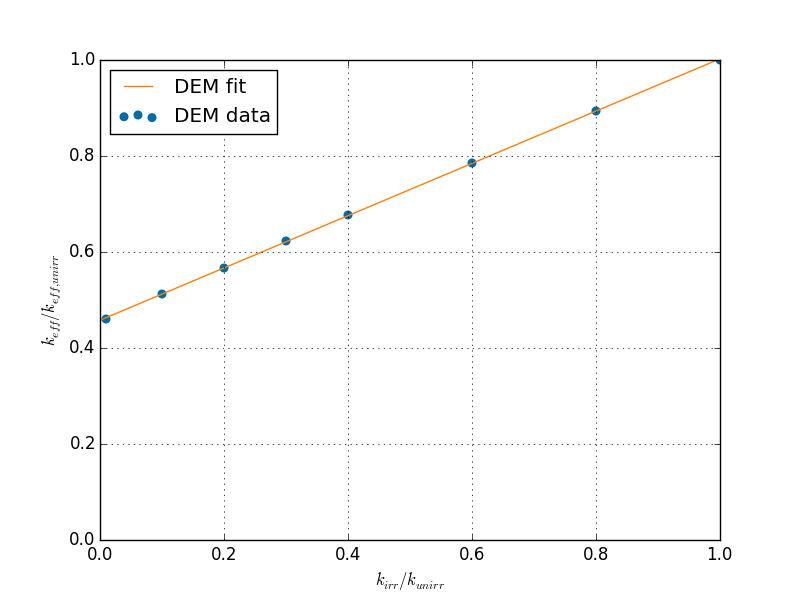
\includegraphics[width = 0.75\textwidth]{figures/irradiated/keff-plots-cfd-q.png}
    \caption{In CFD-DEM-based simulations, $\keff$ of pebble beds decreases linearly with reduced solid conductivity to a limit of $\keff \rightarrow \SI{0.46}{\watt\per\meter\per\kelvin}$ when solid conductivity is reduced.}\label{fig:irrad-keff-cfd-q}
\end{figure}
In the presence of stagnant helium, the effective thermal conductivity is fit to the following linear equation with $R^2 = 0.9998$,
\begin{equation}
\keff [\si{\watt\per\meter\per\kelvin}] = 0.545 \eta + 0.458
\end{equation}
Interestingly, as $k_\text{irr} \rightarrow \SI{0}{\watt\per\meter\per\kelvin}$, interstitial helium causes $\keff \rightarrow \SI{0.46}{\watt\per\meter\per\kelvin}$. Interstitial helium plays a significant role in the ability of the overall pebble bed to transport heat, even when its conductivity (as used in this modeling effort) is only $k_f = \SI{0.34}{\watt\per\meter\per\kelvin}$. Normalized reductions in effective conductivity for irradiated pebbles in DEM and CFD-DEM environments are compared directly in \Cref{fig:irrad-keff-cfd-comparison}. \Cref{fig:irrad-keff-cfd-comparison} shows the contribution of helium at maintaining effective thermal conductivity of pebble beds after the solid material is damaged due to neutron-induced vacancies. Large reductions in solid conductivity, \textit{i.e.} more than one order of magnitude, almost completely destroys the ability of pebbles to transport heat out of the assembly. Interstitial helium provides a limit to how far effective conductivity can drop in beds. We see a linear decrease in effective conductivity at a rate that is half as fast as the linear reduction in solid conductivity; evident from the slope of \num{0.55}.

Plotted in \Cref{fig:irrad-keff-kappa} are the results from our CFD-DEM model plotted alongside much other experimental data from Ref.\cite{VanAntwerpen2010}~as well as the heat transfer correlations for stagnant interstitial gas (discussed in \Cref{sec:keff-correlations}). As a reminder, $\kappa = \frac{k_s}{k_f}$. From \Cref{fig:irrad-keff-kappa}, we see at larger values of solid conductivity, the CFD-DEM results compare well with many correlations from literature. However, for the two smallest values of $\kappa$ (of $k_{irr} = 0.1, 0.01$), the results from CFD-DEM are above theoretical predictions and experimental data by almost double. At $\kappa = 1$, fluid and solid conductivities are equal and as such, the effective thermal conductivity should similarly be unity. The fact that the CFD-DEM results yield data twice as high as theory suggests more investigation is required. 

In mapping Lagrangian data from DEM into Eulerian CFD fields (for \textit{e.g.} calculating porosity and inter-phase exchange coefficients), the divided technique is employed (see \Cref{fig:centroid-void-fraction-divided}). Mapping fluid temperatures back onto DEM, however, employed the simpler particle-centroid technique. A validation effort was performed to define proper fluid mesh sizes in the unirradiated pebble bed condition.

\begin{figure}[ht]
    \centering
    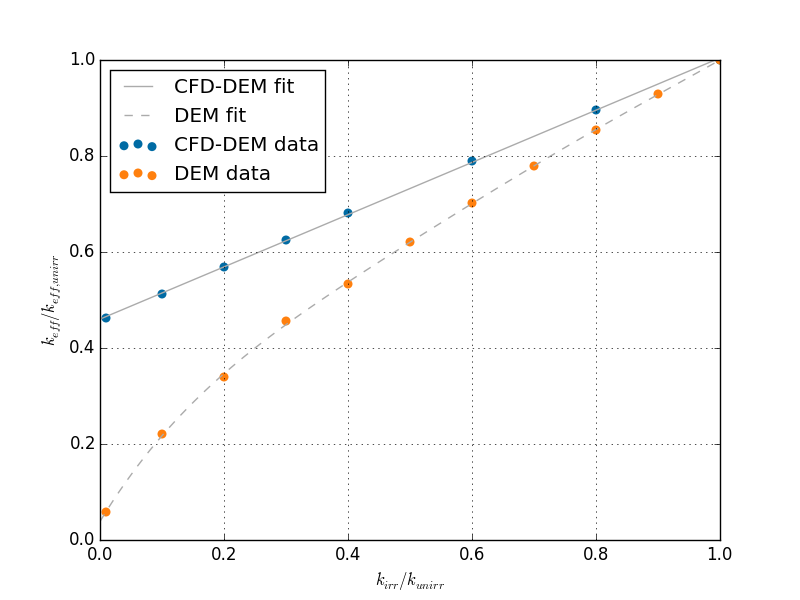
\includegraphics[width = 0.75\textwidth]{figures/irradiated/keff-plots-cfd-comparison.png}
    \caption{Helium's contribution maintains a minimum of $\keff$ even as contact-conductance heat transfer reduces to 0, as demonstrated by $\keff$ of DEM-based results.}\label{fig:irrad-keff-cfd-comparison}
\end{figure}

\begin{figure}[ht]
    \centering
    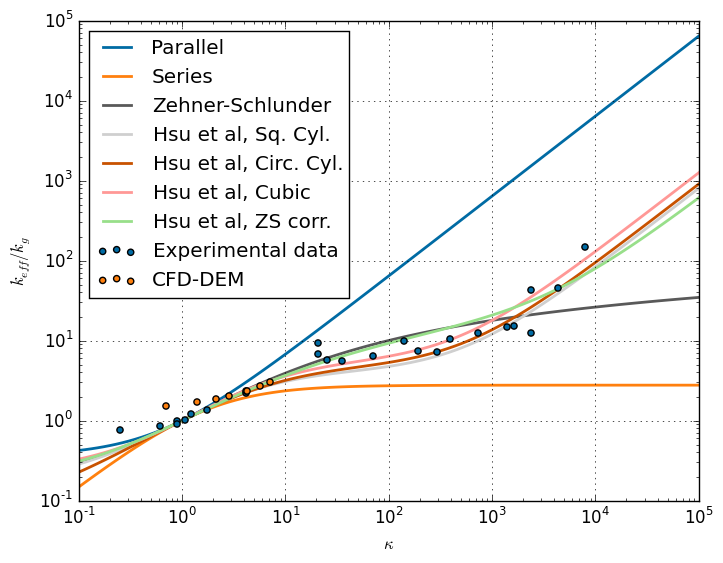
\includegraphics[width = 0.75\textwidth]{figures/irradiated/keff-kappa-irradiated.png}
    \caption{Values of $\keff$ measured for irradiated pebbles with CFD-DEM for all but the smallest solid conductivity values compare well with correlations and other experimental data.}\label{fig:irrad-keff-kappa}
\end{figure}
\FloatBarrier




Again mid-line temperatures for the considered pebble beds are given in \Cref{fig:irrad-mids-cfd-q}.
\begin{figure}[ht]
    \centering
    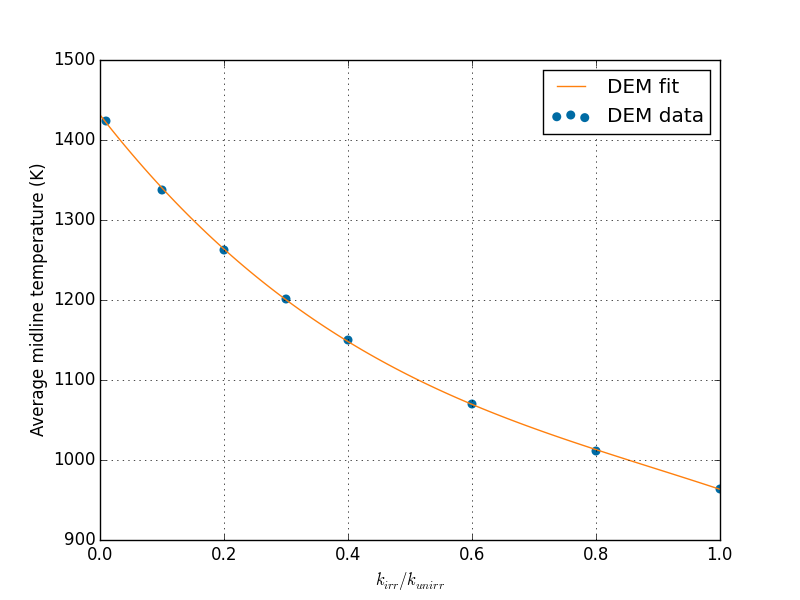
\includegraphics[width = 0.75\textwidth]{figures/irradiated/Tmid-plots-cfd-q.png}
    \caption{In CFD-DEM-based simulations, mid-line temperatures increase as solid conductivity drops; the increase is governed by helium heat transfer continuing in spite of large reductions in solid conductivity.}\label{fig:irrad-mids-cfd-q}
\end{figure}

Data for mid-line temperatures was fit to the following third-order polynomial with $R^2 = 0.9999$ equation,
\begin{equation}
T_\text{mid}[\si{\kelvin}] = -314.1 \eta^3 + 840.1 \eta^2 - 994 \eta + 1431
\end{equation}

In the pebble bed with non-irradiated pebbles, the average maximum temperature in the mid-line was \SI{964}{\kelvin}. Wall temperatures are always held at \SI{573}{\kelvin}. As an example, when neutron damage causes solid conductivity to drop by an order of magnitude, the pebble bed centerline temperature increases to \SI{1337}{\kelvin}, an increase of nearly 40\%. The temperature curves given here are, however, for a generic volume under the average maximum heat generation rate expected for Korean designs of HCPBs, namely \SI{8}{\mega\watt\per\meter\cubed} and no consideration was given for design margins of temperatures in beds. As such, the magnitude of temperature given here may not match design targets of a real blanket. It is thus illustrative to consider a non-dimensional temperature and view its increase. To that end, a second set of pebble beds was run with a nuclear heat rate of \SI{5.12}{\mega\watt\per\meter\cubed}. Maximum bed temperatures are reported in non-dimensional terms; bed temperatures are normalized against the unirradiated result,
\begin{equation}
\Theta = \frac{T_\text{mid}(\eta) - T_\text{wall}}{T_\text{mid,unirr} - T_\text{wall}}
\end{equation}

With this transformation from temperature magnitude, the results of any nuclear heat generation rate or bed geometry will collapse into a single curve, shown in \Cref{fig:irrad-Tmid-cfd-comparison}. The curve is fit with the following relationship
\begin{equation}\label{eq:theta-eta-midline}
\Theta = -0.803 \eta^3 + 2.148 \eta^2 - 2.541 \eta + 2.194
\end{equation}
\begin{figure}[ht]
    \centering
    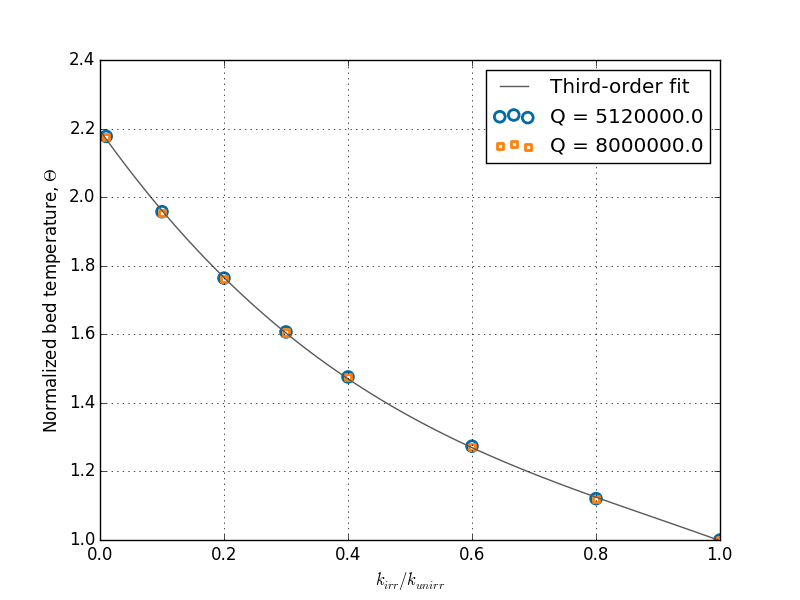
\includegraphics[width = 0.75\textwidth]{figures/irradiated/Tmid-plots-cfd-Tmid-comparison.png}
    \caption{Non-dimensional temperatures of different pebble beds collapse into a single curve, allowing direct comparison of pebble bed temperature increases for irradiated beds with different operating parameters (of nuclear heat rate and geometry).}\label{fig:irrad-Tmid-cfd-comparison}
\end{figure}

As an example of the applicability of these results, suppose we wish to find the amount of irradiated damage is allowable in a ceramic breeder region. In this scenario, a blanket designer chooses to allow a maximum operating temperature with 10\% margin away from \SI{950}{\celsius}. The planned bed mid-line temperature would therefore be \SI{855}{\celsius}. To find the amount of damage allowable within the 10\% margin, we then know $\Theta = \frac{950-573}{855-573} = 1.34$. Thus, solving for $\eta$ in \Cref{eq:theta-eta-midline} yields $\eta = 0.52$; a solid conductivity of $k_{s,irr} = \SI{1.25}{\watt\per\meter\per\kelvin}$. The last step would require knowledge of a relationship between solid conductivity and dpa. With such information, allowable dpa could be ascertained and the 10\% design margin on temperature evaluated.





Neutrons from fusion plasma are highly energetic and it is important to consider how these neutrons will affect heat transport internal to lithium ceramics during their operation in a fusion reactor. In this study, we varied solid thermal conductivity parametrically as a proxy to represent material damaged by neutron irradiation. When stagnant helium gas is included in the calculation, the results fit well within limits of correlations and theoretical limits above $\kappa \approx 1$. We also arrived at correlations relating effective thermal conductivity and maximum bed temperatures as a function of irradiated solid conductivity. At present we have no data indicating the precise quantity of expected dpa in lithium ceramics, nor a correlation between dpa and reduced conductivity. There is, however, irradiation data from a high-dose fission experiment, HICU, in which it appears conductivity values did not decrease dramatically at the temperatures and dpa experienced. Next steps should be to study precisely the relationship between dpa and conductivity in the lithiated ceramic materials considered for use in ITER and future DEMO reactors.

\FloatBarrier












\section{Temperature Distributions with Breeder Orientation, Pebble Fragmentation}\label{sec:isfnt-12}


We apply coupled computational fluid dynamics and discrete element method (CFD-DEM) modeling tools with new numerical implementations of pebble fragmentation to study the combined effects of granular crushing and ensemble restructuring, granular fragment size, and initial packing for different breeder volume configurations. In typical solid breeder modules, heat removal from beds relies on maintaining pebble-pebble and pebble-wall contact integrity. However, contact is disrupted when an ensemble responds to individually-crushed pebbles. Furthermore, restructuring of metastable packings after crushing events are, in part, dependent on gravity forces acting upon the pebbles. We investigate two representative pebble bed configurations under constant volumetric heat sources; modeling heat removed from beds \textit{via} inter-particle conduction, purge gas convection, and contact between pebble beds and containers. In one configuration, heat is removed from at walls oriented parallel to the gravity vector (no gap formation possible); in the second, heat is removed at walls perpendicular to gravity, allowing for the possibility of gap formation between bed and wall. Judging beds on increase in maximum temperatures as a function of crushed pebble amount, we find that both pebble bed configurations to have advantageous features that manifest at different stages of pebble crushing. However, all configurations benefit from achieving high initial packing fractions.



\subsubsection{Simulation domain, boundary conditions, and material properties}

Two ITER-relevant volumes are considered in this study, sketched in \Cref{fig:x-domain,fig:y-domain}. They are differentiated from each other by gravity's direction in the configuration. Because of their similarity, we use generic coordinate systems $(\chi, \zeta)$. Thus $\chi$-configurations, shown in \Cref{fig:x-domain}, have $\chi = y$ and $\zeta = x$ while $\zeta$-configurations, \Cref{fig:y-domain}, have $\chi = x$ and $\zeta = y$. The $\zeta$-configuration in this study is meant to represent the orientation of European Union's TBM \cite{Hernandez2013}, while the $\chi$ configuration is an orientation adopted by many other current TBM designs in ITER \cite{Cho2008,Feng2012a}.

\begin{figure}[!ht]
    \centering
    \begin{subfigure}[b]{0.44\textwidth}
        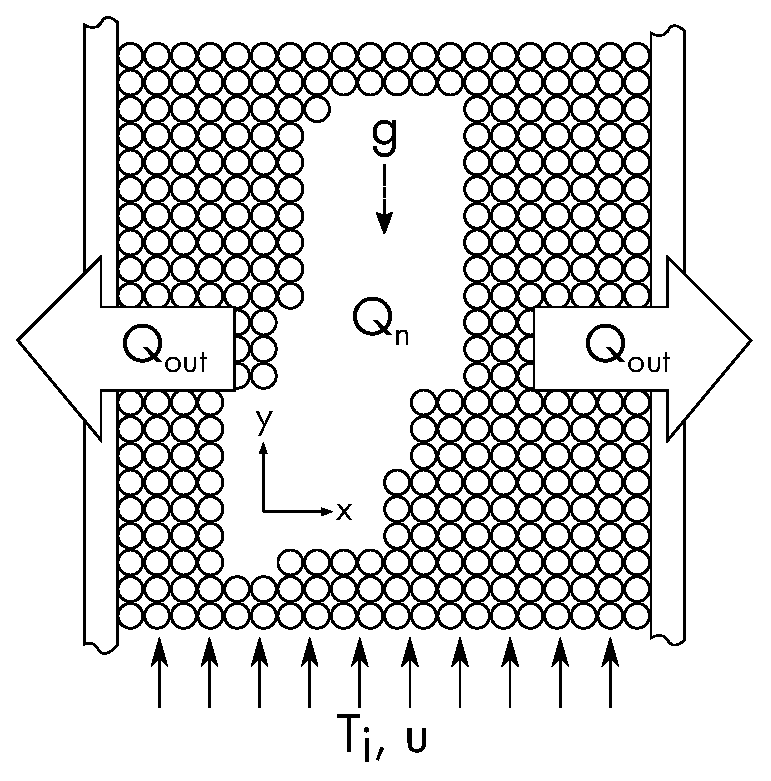
\includegraphics[width = \textwidth]{figures/x-domain.eps}
        \caption{$\chi$-configuration: heat removed in the $x$-direction.}\label{fig:x-domain}
    \end{subfigure}
    ~
    \begin{subfigure}[b]{0.44\textwidth}
        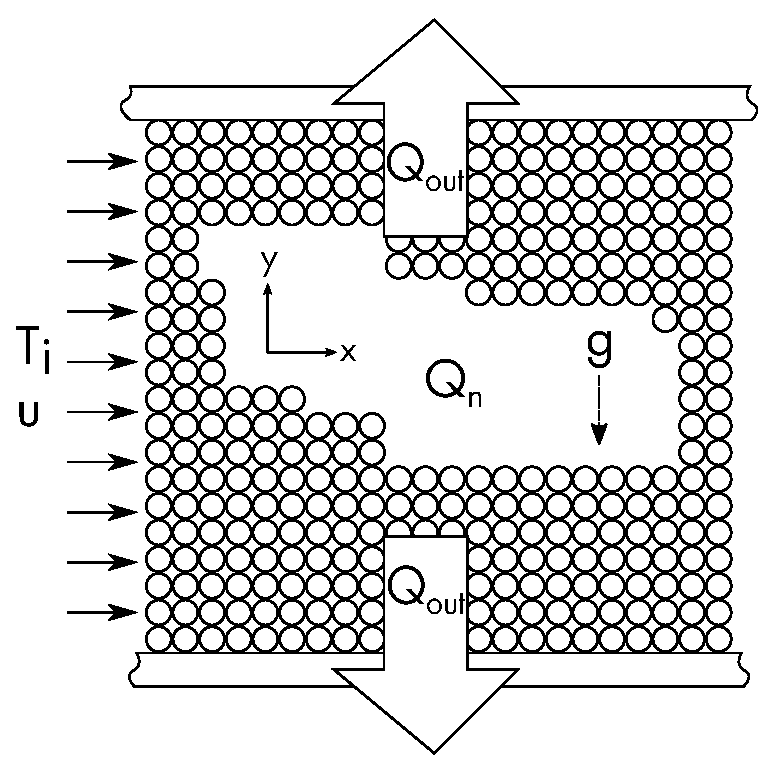
\includegraphics[width = \textwidth]{figures/y-domain.eps}
        \caption{$\zeta$-configuration: heat removed in the $y$-direction}\label{fig:y-domain}
    \end{subfigure}
    \caption{Sketches of the two breeder orientations show that gravity settling will not allow gaps between pebbles and walls in the $\chi$-configuration. However for the $\zeta$-configuration, gravity-induced resettling can create a gap between pebbles and upper wall. }\label{fig:domains}
\end{figure}

In terms of the generic coordinates, outflow of bed heat to coolant is along $\zeta$. Constant temperature boundaries, $T_w$, exist at the edges of that dimension. As sketched in \Cref{fig:domains}, gravity resettling in the $\chi$ configuration will not allow gap formation between bed and wall. However, in the $\zeta$-config it is possible for a gap to form between top coolant walls and pebbles after gravity resettling. A constant nuclear heat rate was applied to every particle in the bed which is representative of the highest source term anticipated in current ITER designs of solid breeder blankets, $q''' = \SI{8e6}{\watt\per\meter\cubed}$.

The simulation consists of pebbles of diameter $d_p = \SI{1}{\milli\meter}$, in beds filled to two initial packing fractions, $\phi_{1,2} = 62, 64\%$. Mechanical properties of the pebbles are given in \Cref{tab:peb-props}. To note is the elastic modulus chosen for pebbles in this study. In a past experimental study, Van Lew \textit{et al}. found that individual pebbles behaved in a manner indicative of having a elastic modulus from 20 to 60\% of values reported in literature for sintered blocks of \lit~and \lis~\cite{VanLew2015}. Therefore to maintain some generality to this study, we have chosen a elastic modulus at a nominal value of $E=\SI{60}{\giga\pascal}$ to generically represent either ceramic pebble.

Pebble bed widths in $\zeta$ are \SI{20}{\milli\meter}, a size comparable to breeding volumes of many ITER TBM designs \cite{Hernandez2013,Cho2008,Feng2012a}. Bed depths (in the $z$-direction, in/out of the page in \Cref{fig:x-domain,fig:y-domain}) are \SI{5}{\milli\meter}, with periodic boundary conditions. Bed lengths in $\chi$ vary to accommodate \SI{6000} pebbles, initially, with given initial packing fractions; the length is approximately \SI{50}{\milli\meter}. Virtual walls are placed at extents of $\chi$ and $\zeta$ dimensions. Walls in $\zeta$ had constant temperature boundaries of $T_{w,s}$, all walls have mechanical and thermal properties of structural steel, given in \Cref{tab:wall-props}.

Fluid domains, overlaid on DEM pebbles, have fluid inlet and outlet regions of lengths \SI{10}{\milli\meter} and approximately \SI{51}{\milli\meter}, respectively. The side walls of the fluid domain were adiabatic in inlet and outlet regions and had constant temperature boundaries where they contacted the pebble bed, $T_{w,f}$. Fluid entered with a constant velocity magnitude of \SI{5}{\centi\meter\per\second} and constant temperature $T_i$. At present, temperature-dependencies of helium properties have not been incorporated into the model. Over the range of \SIrange{400}{900}{\celsius}, increases in helium momentum and thermal diffusivities are both essentially linear and thus an arithmetic mean for properties over that range is used as a first approximation. Future models will incorporate temperature-dependence of fluid properties. Fluid transport properties are given in \Cref{tab:fluid-props}. 
%---------------------------------------------------------------------------------------
% FIGURES
%---------------------------------------------------------------------------------------
% \begin{figure*}[!ht]
%        \centering
%        \begin{subfigure}[b]{0.45\textwidth}
%                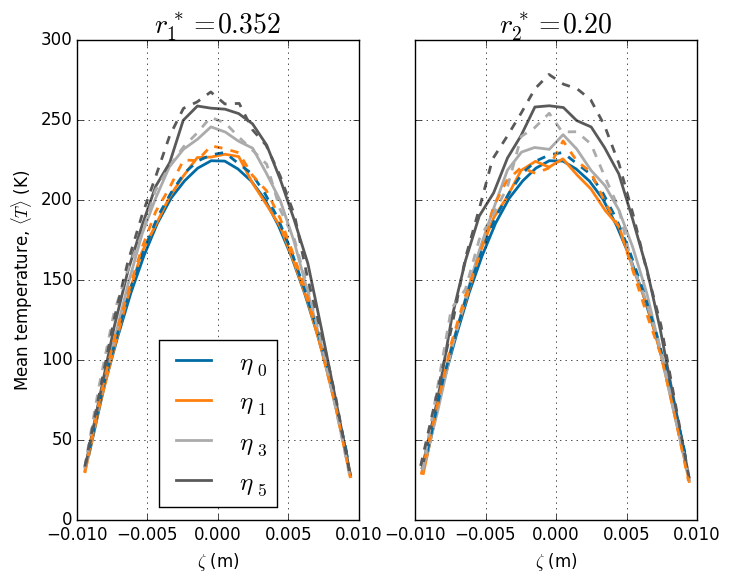
\includegraphics[width=\textwidth]{figures/62-percent-T-profiles.png}
%                \caption{Initial packing fraction of $\phi_1 = 0.62$.}
%                \label{fig:62-T-profile}
%        \end{subfigure}%
%        ~ %add desired spacing between images, e. g. ~, \quad, \qquad, \hfill etc.
%          %(or a blank line to force the subfigure onto a new line)
%        \begin{subfigure}[b]{0.45\textwidth}
%                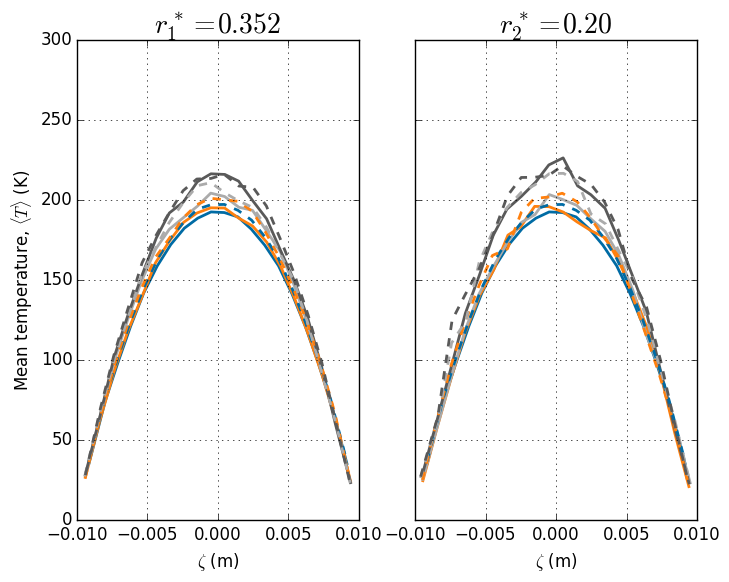
\includegraphics[width=\textwidth]{figures/64-percent-T-profiles.png}
%                \caption{Initial packing fraction of $\phi_2 = 0.64$.}
%                \label{fig:64-T-profile}
%        \end{subfigure}
%        \caption{Solid lines are cases where gravity is in the $\chi$ direction, dashed lines for gravity in the $\zeta$ direction; color is by percent of crushed pebbles, $\eta$.}
% \label{fig:T-profiles}
% \end{figure*}


%---------------------------------------------------------------------------------------
% TABLES
%---------------------------------------------------------------------------------------
\begin{table}[ht]
\centering
\caption{Mechanical and thermal properties of ceramic pebbles in the DEM domain. Aside from $E_s$, properties come from \cite{Gierszewski1998} with $\epsilon = 0.2$}
\label{tab:peb-props}
\resizebox{0.45\textwidth}{!}{%
\begin{tabular}{@{}lcS[table-format=3.2]@{}}
\toprule
%properties are coming from the lit_props.py file in the thesis scripts folder. Double check if you want
Property                                           & Symbol    & \text{Value} \\ \midrule
elastic modulus (\si{\giga\pascal})                & $E_s$     & 60.    \\
Poisson ratio                                      & $\nu_s$     & 0.24  \\
thermal conductivity (\si{\watt\per\meter\per\kelvin}) & $k_s$     & 1.79   \\
diameter (\si{\meter})                             & $d_p$     & 0.001     \\
pebble-pebble friction coefficient                 & $\mu_s$   & 0.2   \\
pebble-wall friction coefficient                   & $\mu_w$   & 0.2   \\ 
heat capacity (\si{\joule\per\kilo\gram\per\kelvin})   & $c_{s}$     & \num{1.45e3}  \\
thermal expansion coefficient (\si{\per\kelvin})   & $\beta_s$ & \num{1.77e-5}      \\
density (\si{\kilo\gram\per\cubic\meter})          & $\rho_s$  & \num{3.44e3}  \\ \bottomrule
\end{tabular}}
\end{table}

\begin{table}[ht]
\centering
\caption{Mechanical and thermal properties and boundary conditions of structural container in the DEM domain \cite{Fokkens2003}.}
\label{tab:wall-props}
\resizebox{0.45\textwidth}{!}{%
\begin{tabular}{@{}lcS[table-format=3.2]@{}}
\toprule
Property                                           & Symbol    & \text{Value} \\ \midrule
elastic modulus (\si{\giga\pascal})                & $E_w$     & 175.    \\
Poisson ratio                                      & $\nu_w$     & 0.30  \\
thermal conductivity (\si{\watt\per\meter\per\kelvin}) & $k_w$     & 29.0   \\ 
wall temperature (\si{\kelvin})                     & $T_{w,s}$        & 573    \\ \bottomrule
\end{tabular}}
\end{table}

\begin{table}[ht]
\centering
\caption{Transport properties of helium and boundary conditions in the CFD domain; mean values over the temperature range \SIrange{400}{900}{\celsius}.}
\label{tab:fluid-props}
\resizebox{0.45\textwidth}{!}{%
\begin{tabular}{@{}lcl@{}}
\toprule
% properties in excel sheet in thesis scripts folder
Property                                           & Symbol    & \text{Value} \\ \midrule
thermal conductivity (\si{\watt\per\meter\per\kelvin}) & $k_f$     & \num{3.40e-1}   \\
heat capacity (\si{\joule\per\kilo\gram\per\kelvin})   & $c_{f}$     & \num{5.19e3}  \\
density (\si{\kilo\gram\per\cubic\meter})          & $\rho_f$  & \num{5.38e-2}  \\
kinematic viscosity (\si{\meter\per\second\squared})   & $\lambda_f$ & \num{8.52e-4}      \\ 
thermal diffusivity (\si{\meter\per\second\squared})   & $\alpha_f$ & \num{1.28e-3}      \\ 
wall temperature (\si{\kelvin})                     & $T_{w,f}$        & 573    \\ 
inlet temperature (\si{\kelvin})                    & $T_i$            & 573    \\ \bottomrule
\end{tabular}}
\end{table}



\subsubsection{Modeling crush events}
Models have been proposed in the past which translate experimental measurements of granular crushing into contact forces in an ensemble to predict granular crushing, \textit{e.g.} Refs.~\cite{Gan:2010kc,Russell2009,Zhao2012,VanLew2015,Annabattula2014}, but no validation has set any model apart as yet. Here, packed beds experience artificial pebble-crushing events for which a chosen percentage, $\eta$, of initial pebbles (at randomized locations) fragment. Four pebble crush percentages are used: $\eta = 0, 1, 3, 5\%$. Numerical models of crush events themselves have received attention. Annabattula, Zhao, and Gan attempted to model a crushing event as either a reduction in radius of the crushed pebble or a reduction in elastic modulus \cite{Annabattula2011,Zhao2013,Annabattula2012a}. Van Lew \textit{et al}~made similar simplifications when they considered a crushed pebble as being removed from the force network, thus being removed from the DEM domain \cite{VanLew2014}. 

%None of the approaches discussed above have been fully validated due to a lack of experimental results. 
In this work, we replace a parent pebble of radius $r$ with $N_c$ smaller daughter fragments, each of equal radius, $r_c$. After a crushing event, fragments are free to resettle through interstitial gaps in the pebble bed and original pebbles respond in kind with re-arrangement into a new metastable packing structure.  To conserve volume between pre- and post-crush, we can relate the number of daughter fragments to the radius ratio between fragments and parent, $r^* = r_c/r$, as $N_c = (1/r^*)^{3}$. Conservation of energy of crush events is enforced by setting the temperature of daughter fragments equal to the parent pebble at the moment of crushing. 

Numeric techniques to handle overlap after crush events, as a consequence of volume conservation, were shown in \Cref{sec:failure-study}. To summarize the approach, in our fragmentation procedure, overlap and the associated high contact forces between the daughter fragments is permitted. Directly following a fragmentation event, a cut-off distance is applied to the velocity-Verlet integration of daughter fragments which prevents instabilities in position; \textit{e.g.} in any given timestep fragments are only allowed to travel $x_\text{cutoff}$, regardless of the distance calculated in integration. A short time is permitted for the daughter fragments to relax away from the highly-overlapped state; relaxation time was a function of number of pebble fragments and pebble fragment size. Contact forces in the system were monitored and when average values returned to pre-fragmentation levels, the relaxation procedure concluded, cut-off distance was removed, and standard velocity-Verlet integration of daughter pebbles was reinstated.

Experimental studies of crushing brittle pebbles show many different modes of fragmentation, often with highly irregular sizes (see \textit{e.g.} Ref.\cite{Wu2004}). As a first effort, we compare the effect of fragmentation size by studying two different values, $r^*_1 = 0.32$ and $r^*_2 = 0.2$ which results in $N_{c,1} = 23$ and $N_{c,2} = 125$ daughters per crushed parent (at $\eta = 5\%$, for $r_2^*$ the system expands to \num{43200} pebbles). 









\subsection{Results \& Discussion}
In \Cref{fig:inset}, a bed of 64\% initial packing with 5\% of pebbles broken into fragments of size $r_2^* = 0.2$ is shown; vectors of flow field, colored by fluid temperature, are seen moving through the bed. The inset image qualitatively demonstrates how the fluid field aids in equilibrating temperatures of fragments with neighboring larger pebbles in spite of light physical contact between pebbles. 

\begin{figure}[ht]
    \centering
    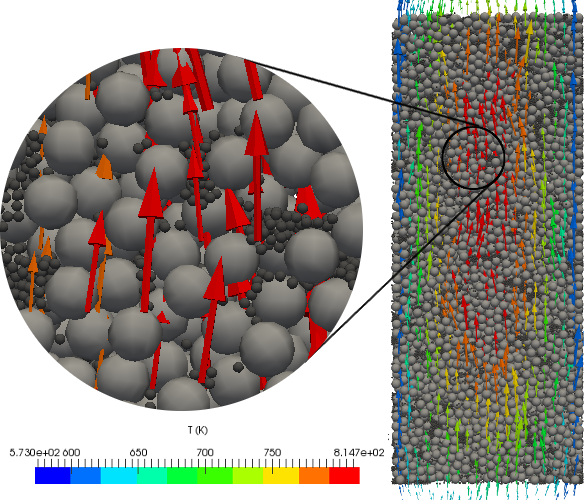
\includegraphics[width = 0.75\textwidth]{figures/pebble_inset_2.png}
    \caption{Showing the case for $\phi_2 = 0.64$, $\eta = 5\%$ with fluid velocity vectors colored by temperature. Inset image reveals size discrepancies between fragments and pebbles and the ensemble interaction with fluid flow.}\label{fig:inset}
\end{figure}

Several cross-sections are created at mid-planes in $z$. Representative results are taken from 64\% packings of $\zeta$- and $\chi$-configurations and compared against their respective $\eta = 5\%$, $r_2^*$ conditions, shown in \Cref{fig:1,fig:3}. The numbered zones of the beds will be discussed shortly.

\begin{figure}[!ht]
    \centering
    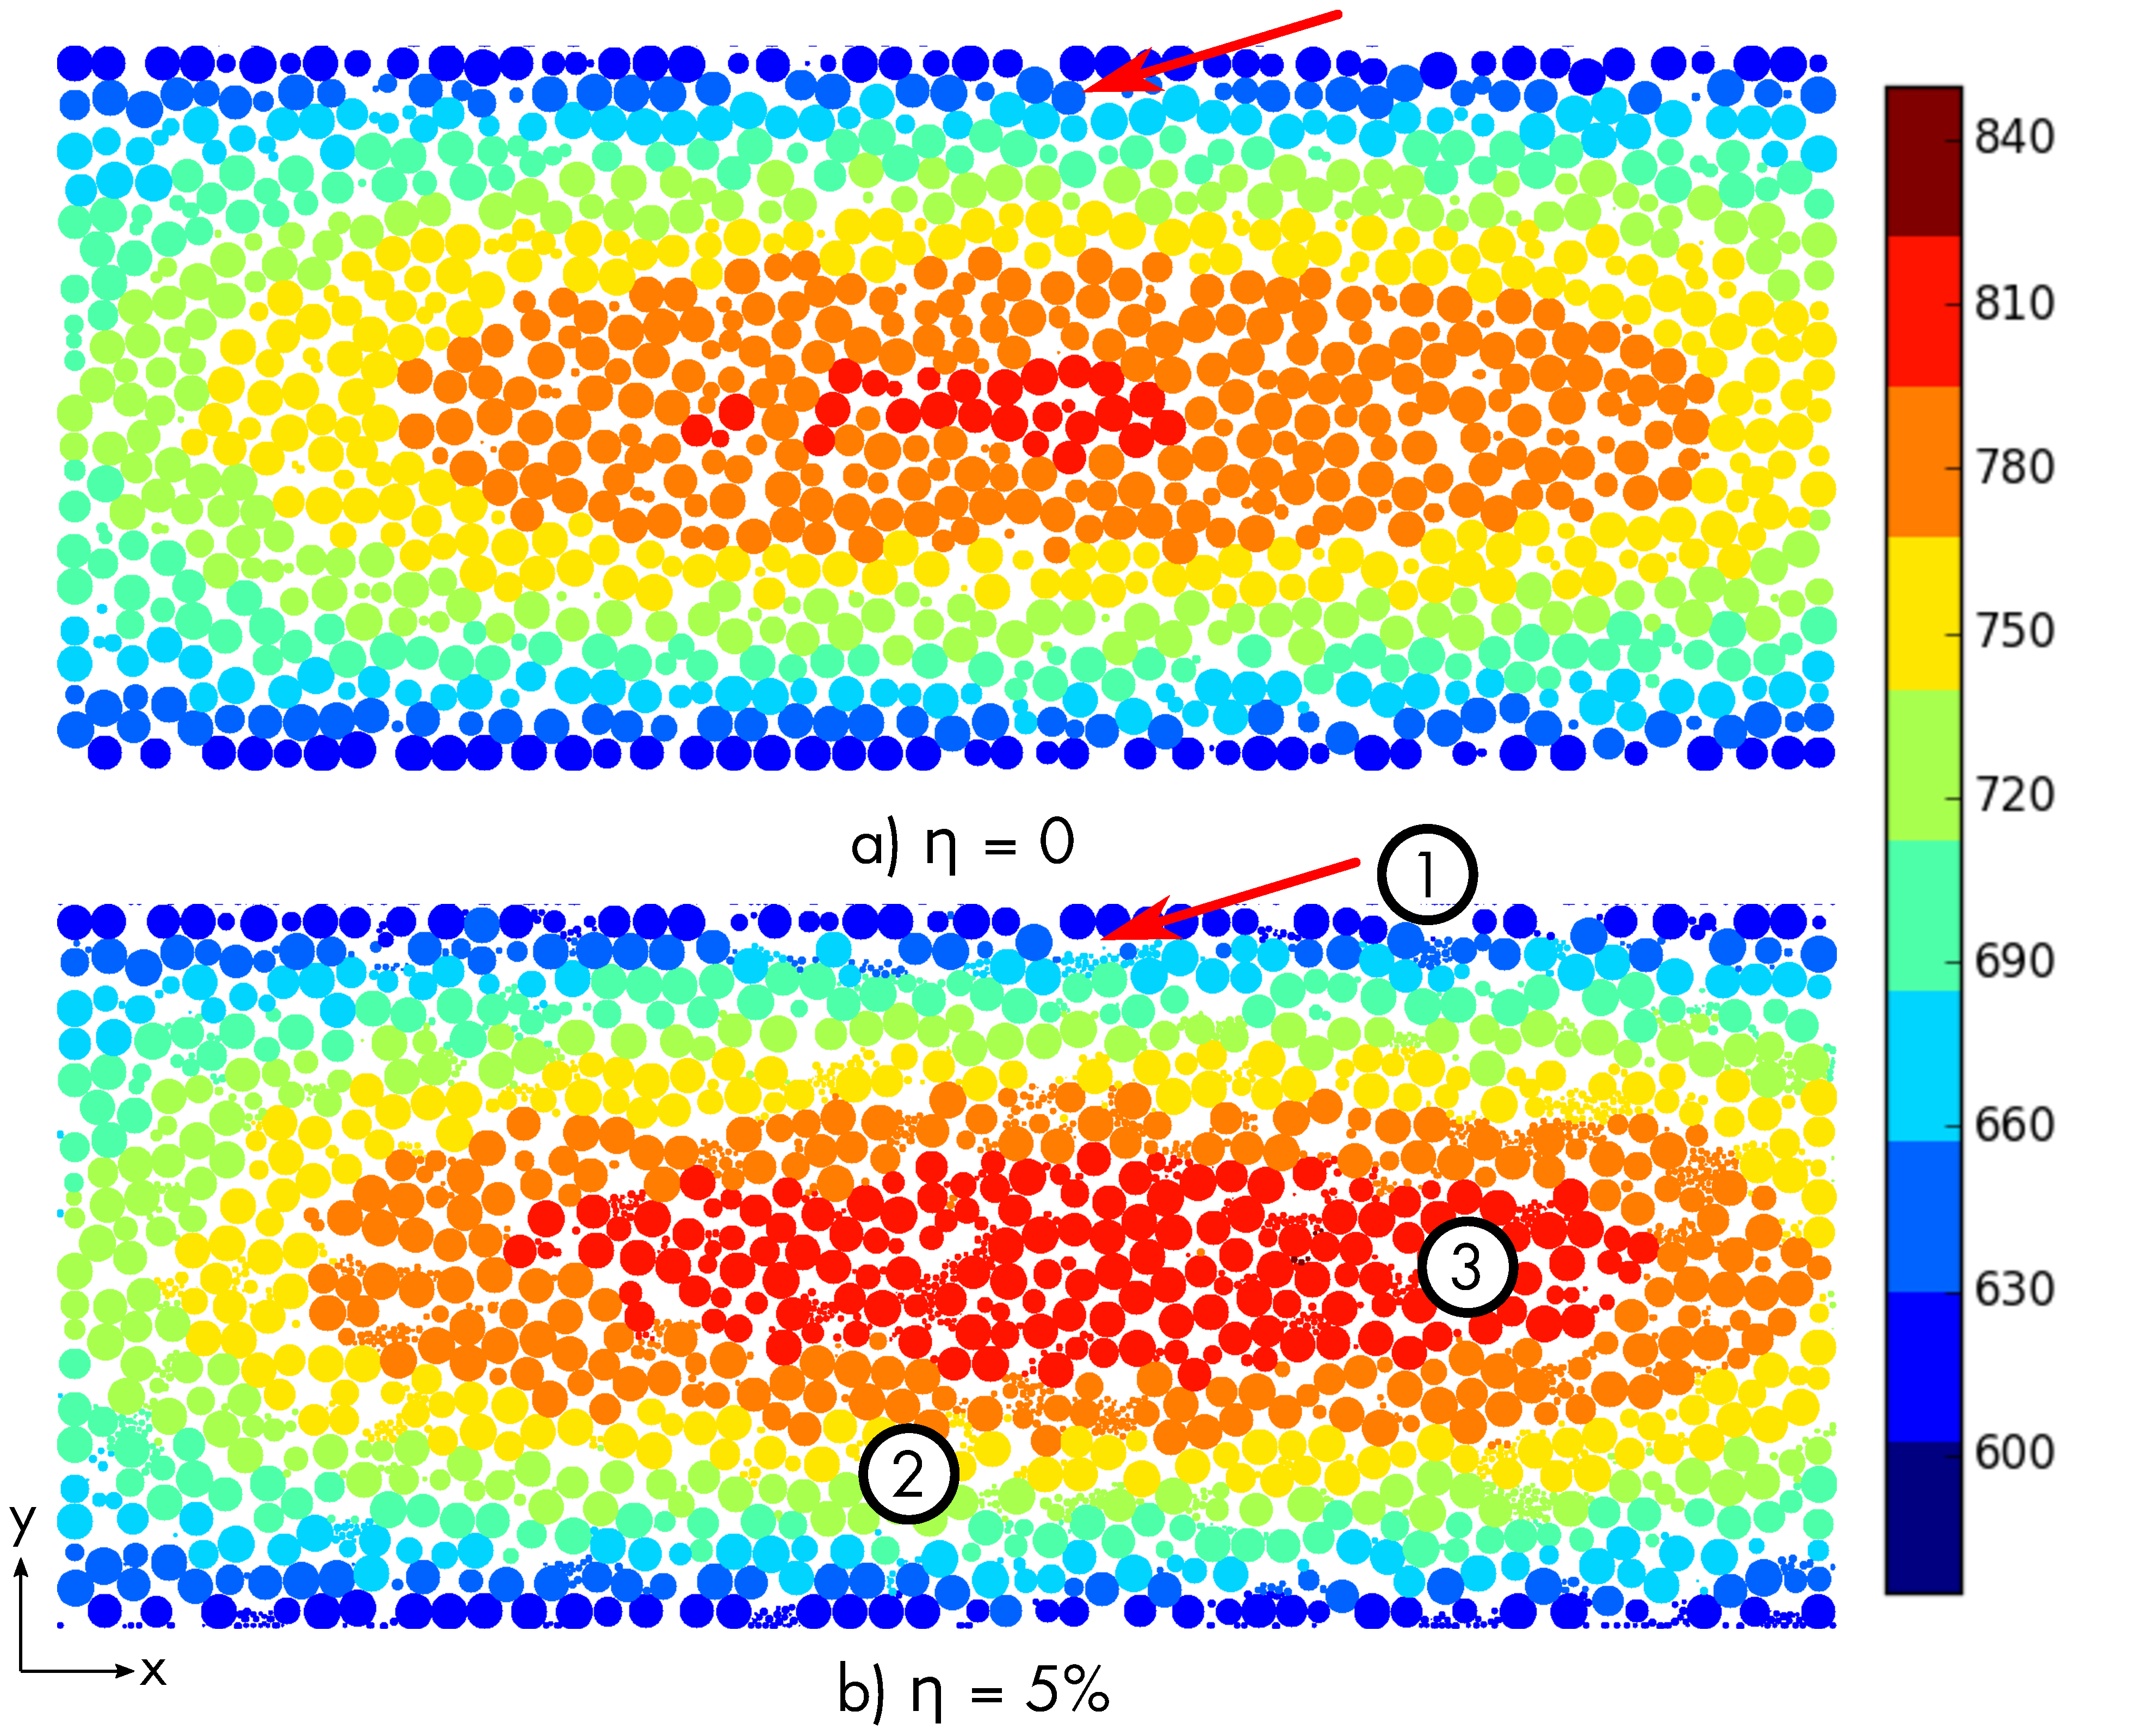
\includegraphics[width = \textwidth]{figures/z-64-discrete.eps}
    \caption{Cuts at the mid-plane of $z$ for $\zeta$-config beds. (a) bed initially packed to $\phi_2$, and (b) bed with crushing of $\eta_5$ pebbles with particle size $r_2^*$.}\label{fig:1}
\end{figure}

\begin{figure}[!ht]
    \centering
    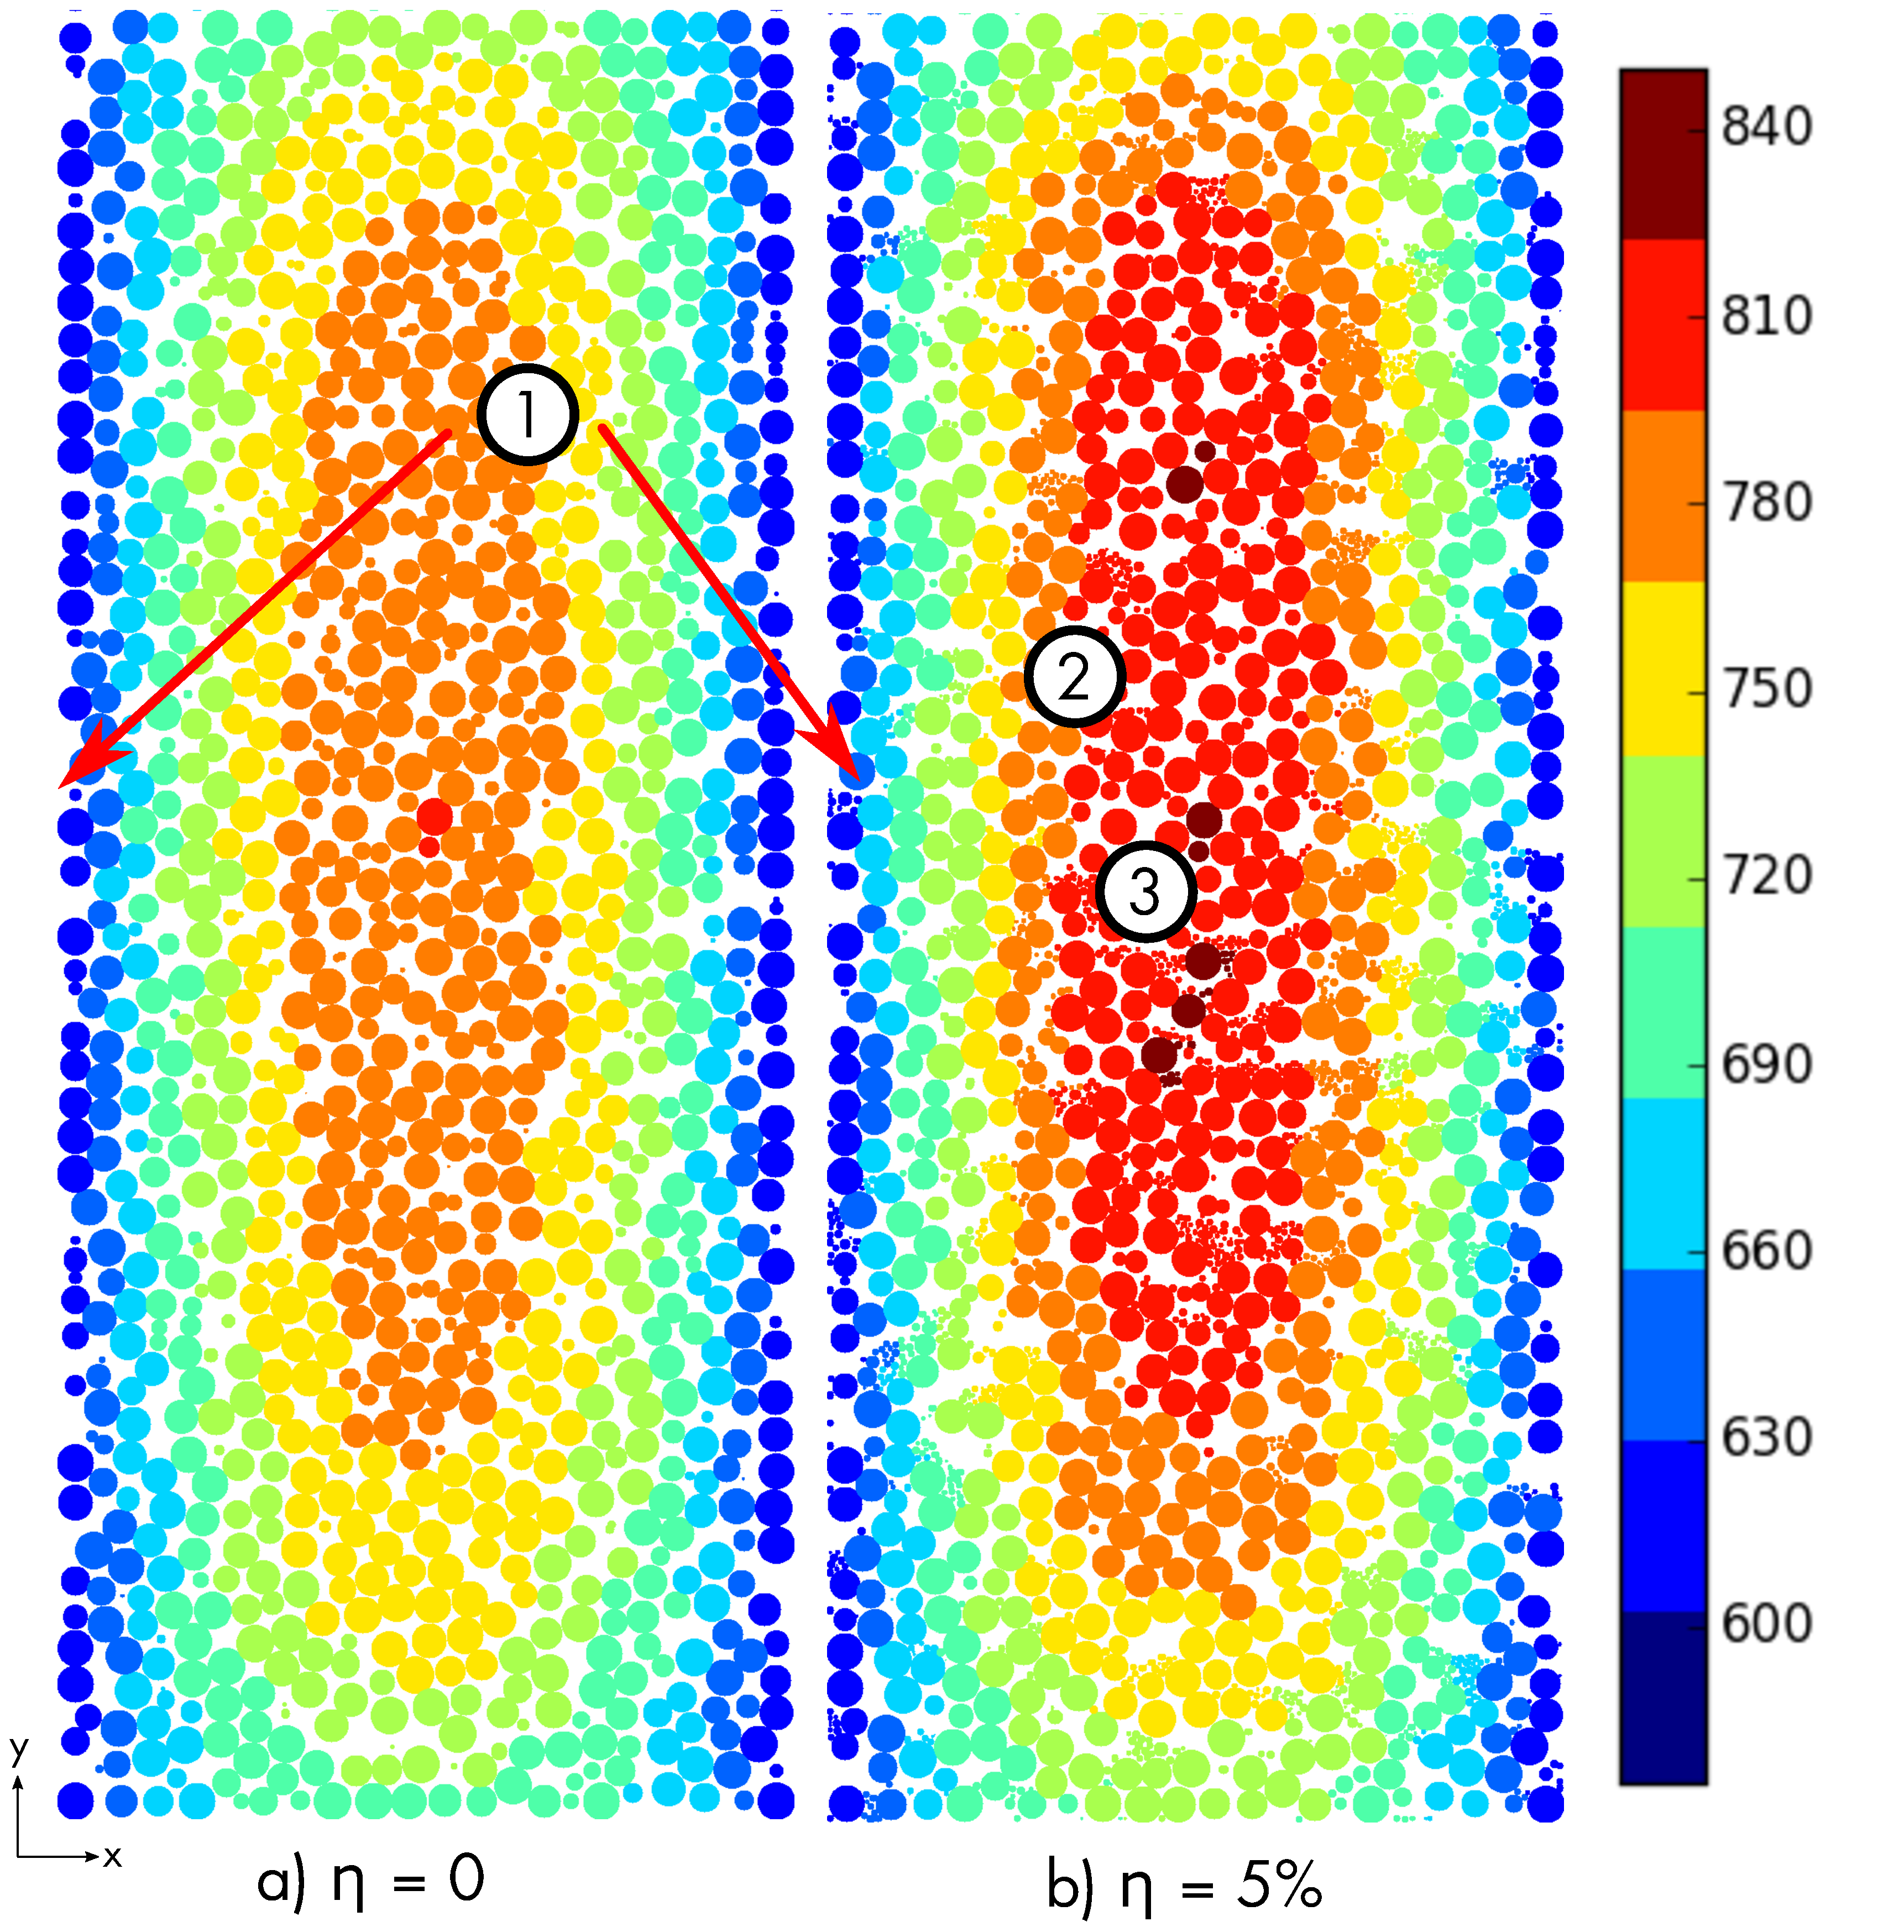
\includegraphics[width = 0.75\textwidth]{figures/x-64-discrete.eps}
    \caption{Cuts at the mid-plane of $z$ for $\chi$-config beds. (a) bed initially packed to $\phi_2$, and (b) bed with crushing of $\eta_5$ pebbles with particle size $r_2^*$.}\label{fig:3}
\end{figure}

Wall offset temperatures ($T-T_w$) in beds are found in slices of width $\Delta\zeta$ along $\zeta$. Pebble-weighted mean values are found as $\langle T\rangle = \frac{1}{V_n}\sum_{j}^n (T_j-T_w) V_j$, for $n$ pebbles of temperature $T_j$ consuming a total volume $V_n$ in the slice. Demonstrative cases of $\phi_2 = 0.64$ with $r_2^* = 0.2$ are given in \Cref{fig:64-T-profile} as functions of granular crushing percentage.

We report the overall hydrostatic pressure of pebble beds, $p = \sigma_{ii}/3$, at steady-state heating. Bed stress tensors can be calculated as\cite{Martin2004,Gan:2010uq,An20072233}, 
\begin{equation}
\bm{\sigma} = \frac{1}{V}\left(\sum^{N} \delta_{ij} f_{n,ij} \vec{n}\otimes\vec{n} + \sum^{N} \delta_{ij}f_{t,ij} \vec{n}\otimes\vec{t}\right)
\end{equation}
where $\vec{n}$ and $\vec{t}$ are unit vectors of the normal and tangential directions, respectively, and $f_n$ and $f_t$ are the magnitudes of force in the normal and tangential directions, respectively. Hydrostatic pressure values are normalized against initial ($\eta=0$) beds for respective configurations. Hydrostatic pressure is given in \Cref{fig:eta-sigma}.%considered configuration, $\sigma^*=|\sigma|_\eta/|\sigma|_{\eta_0}$. %Normalized bed stresses decrease with increasing granular fragmentation, as seen in \Cref{fig:eta-sigma}, for all initial packings and bed orientations, by about 30 to 60\%.

A total mean bed temperature is found from all pebbles in the system as $\langle T\rangle_{tot} = \frac{1}{V_N}\sum_{j}^N (T_j-T_w) V_j$ where $N$ is the total number of ensemble pebbles. The total mean bed temperature is also normalized against initial packing cases of each respective set of beds. Results for all beds are given in \Cref{fig:eta-theta}. Maximum temperature rises of every bed are also found, $T_m = \max(T) - T_w$, and normalized against the maximum temperature in the initial packing of each respective set of beds. To avoid aberrant results from a bed which might have a single, very high temperature pebble, the maximum temperature, $\max(T)$, is calculated as a mean value of the 50 highest temperature pebbles. The results are given in \Cref{fig:eta-T_max}. In addition to total mean bed temperature, maximum temperature rise is also an important factor in evaluation of a pebble bed.

Lastly, we consider how far pebble fragments travel in the bed after a crushing event. Total displacements from the moment of crush event to final resting, $|\Delta h|$, are normalized against the original pebble diameter, $|\Delta h|/d_p$. Histograms for 64\% packing fractions of $\chi$- and $\zeta$-configurations at 5\% pebble crushing with fragment sizes $r_2^*$ are given in \Cref{fig:displacement_hists}. These two beds saw the most settling, all other beds tested saw considerably less fragment travel.





% \begin{figure}[ht]
% \centering
% 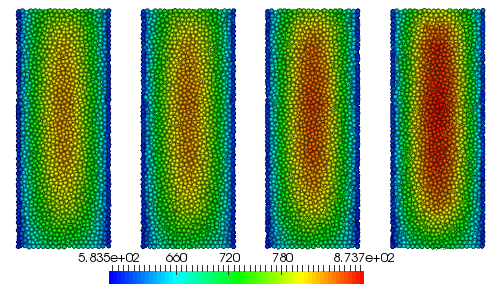
\includegraphics[width = 0.4\textwidth]{figures/62x-edit.png}
% \caption{Pebble temperature distributions in the $\chi$-config with $\phi_1 = 0.62$ initial packing increase with increased granular damage, from left to right is $\eta = 0, 0.01, 0.03, 0.05$.}\label{fig:62xpebs}
% \end{figure}

% numeric integration of mean temperature profiles, $\Theta = \frac{1}{L}\int\langle T \rangle \,\mathrm{d}\zeta$, where $L$ is the \SI{20}{\milli\meter} width of $\zeta$; $\Theta$ is plotted in \Cref{fig:eta-theta}.



% \begin{figure*}[!ht]
%        \centering
%        \begin{subfigure}[b]{0.45\textwidth}
%                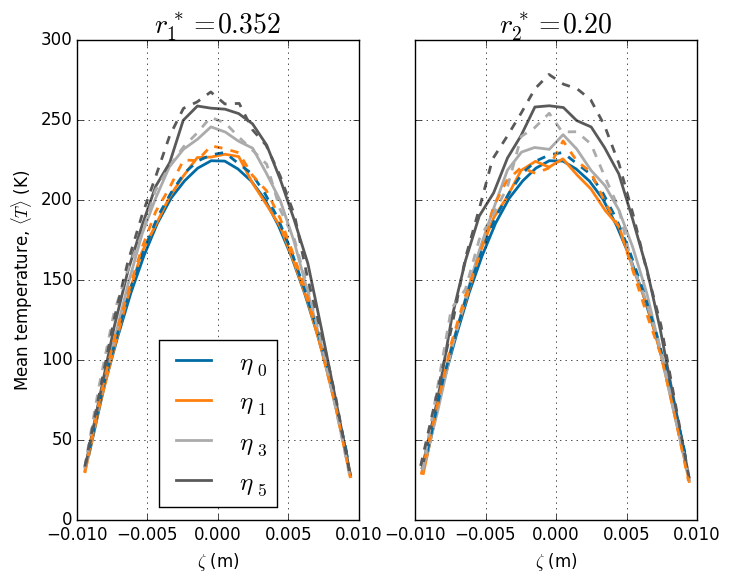
\includegraphics[width=\textwidth]{figures/62-percent-T-profiles.png}
%                \caption{Initial packing fraction of $\phi_1 = 0.62$.}
%                \label{fig:62-T-profile}
%        \end{subfigure}%
%        ~ %add desired spacing between images, e. g. ~, \quad, \qquad, \hfill etc.
%          %(or a blank line to force the subfigure onto a new line)
%        \begin{subfigure}[b]{0.45\textwidth}
%                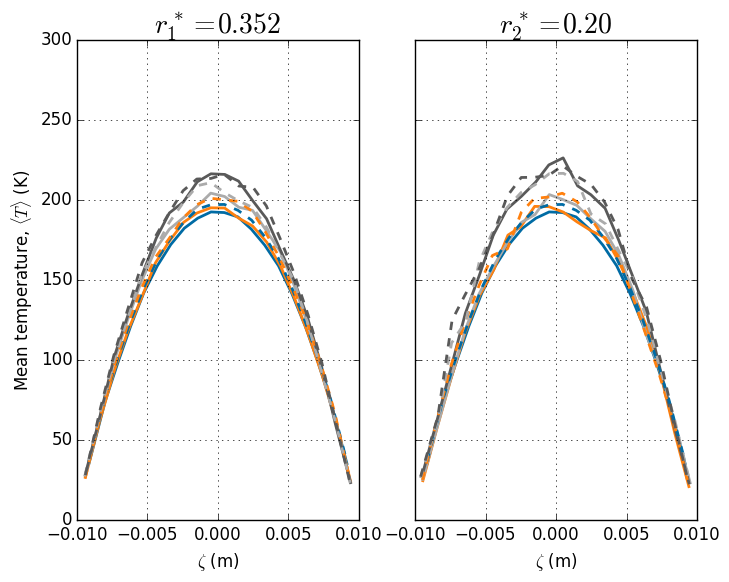
\includegraphics[width=\textwidth]{figures/64-percent-T-profiles.png}
%                \caption{Initial packing fraction of $\phi_2 = 0.64$.}
%                \label{fig:64-T-profile}
%        \end{subfigure}
%        \caption{Solid lines are cases where gravity is in the $\chi$ direction, dashed lines for gravity in the $\zeta$ direction; color is by percent of crushed pebbles, $\eta$.}
% \label{fig:T-profiles}
% \end{figure*}

%

% \begin{figure*}[!ht]
%        \centering
%        \begin{subfigure}[b]{0.45\textwidth}
%                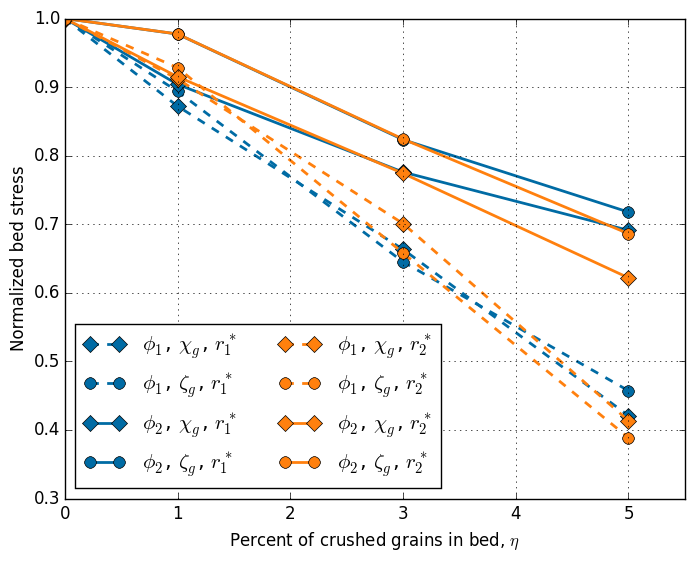
\includegraphics[width = \textwidth]{figures/eta-sigma.png}
%               \caption{Lower packing fractions have lower initial bed stress, stress decreases with increased granular crushing. }\label{fig:eta-sigma}
%        \end{subfigure}%
%        ~ %add desired spacing between images, e. g. ~, \quad, \qquad, \hfill etc.
%          %(or a blank line to force the subfigure onto a new line)
%        \begin{subfigure}[b]{0.45\textwidth}
%                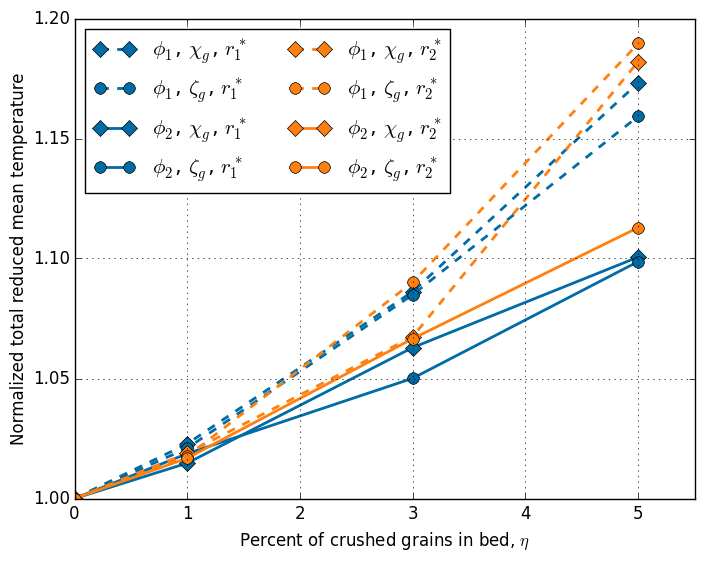
\includegraphics[width = \textwidth]{figures/eta-theta.png}
%               \caption{Lower packing fractions have higher initial bed temperatures, mean temperatures increase with increased granular crushing.}\label{fig:eta-theta}
%        \end{subfigure}
%        \caption{Changes in temperature and bed stress as functions of granular damage percent, $\eta$, with varying parameters of packing fraction, $\phi_1 = 0.62$, $\phi_2 = 0.64$; fragmentation radius ratio, $r_1^* = 0.52$, $r_2^* = 0.2$; and configuration, $\chi_g$ is $\chi$-config, $\zeta_g$ is $\zeta$-config.}
% \label{fig:eta-plots}
% \end{figure*}


\begin{figure}[!t]
    \centering
    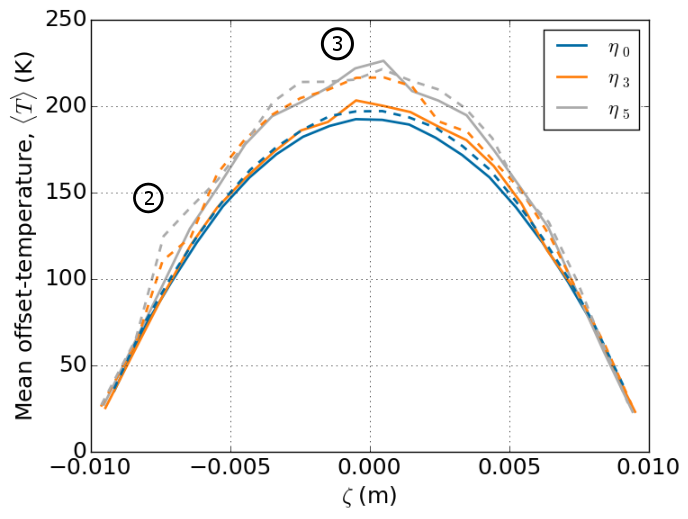
\includegraphics[width=0.65\textwidth]{figures/64-percent-T-profiles-reduced.png}
    \caption{Mean offset temperature profiles, $\langle T \rangle$, along $\zeta$ in beds with initial packing fractions $\phi_2 = 0.64$, fragmentation sizes were $r_2^*$. Solid lines are $\chi$ configurations, dashed lines are $\zeta$ configurations. Fragmentation settling of $\zeta$-configs are seen in `lumps' near Zone (2) and in the $\chi$-config spike in zone (3).}
    \label{fig:64-T-profile}
\end{figure}

\begin{figure}[!t]
    \centering
    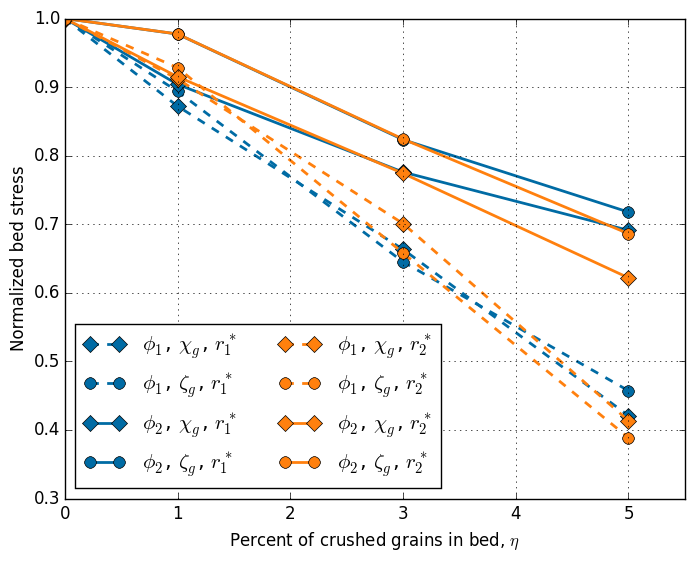
\includegraphics[width = 0.65\textwidth]{figures/eta-sigma.png}
    \caption{Dashed lines represent the lower packing fraction, $\phi_1 = 0.62$, solid lines are $\phi_2 = 0.64$. Markers are: $\circ$ for $\zeta$-config, $\diamondsuit$ for $\chi$-config. Color differentiates the fragment radius ratio. Contact force relaxation is more rapid for lower packing fractions.}\label{fig:eta-sigma}
\end{figure}

\begin{figure}[!t]
    \centering
    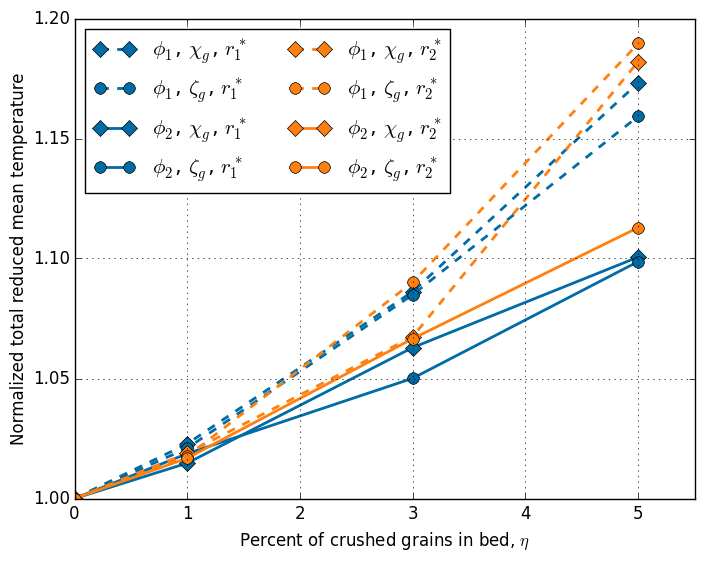
\includegraphics[width = 0.65\textwidth]{figures/eta-theta.png}
    \caption{Dashed lines represent the lower packing fraction, $\phi_1 = 0.62$, solid lines are $\phi_2 = 0.64$. Markers are: $\circ$ for $\zeta$-config, $\diamondsuit$ for $\chi$-config. Color differentiates the fragment radius ratio. Lower packing fraction is the most dominant parameter for overall bed temperature. Amongst the same packing fraction, fragment size is most influential factor.}\label{fig:eta-theta}
\end{figure}

\begin{figure}[!t]
    \centering
    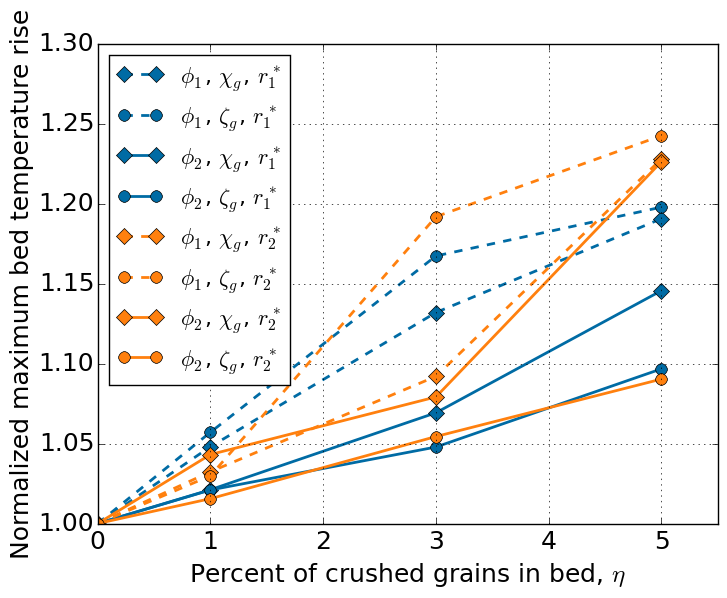
\includegraphics[width = 0.65\textwidth]{figures/eta-T_max.png}
    \caption{Dashed lines represent the lower packing fraction, $\phi_1 = 0.62$, solid lines are $\phi_2 = 0.64$. Markers are: $\circ$ for $\zeta$-config, $\diamondsuit$ for $\chi$-config. Color differentiates the fragment radius ratio. The dominant parameter influencing maximum bed temperature varies as a function of the number of crushed pebbles in the bed.}\label{fig:eta-T_max}
\end{figure}

\begin{figure}[!t]
    \centering
    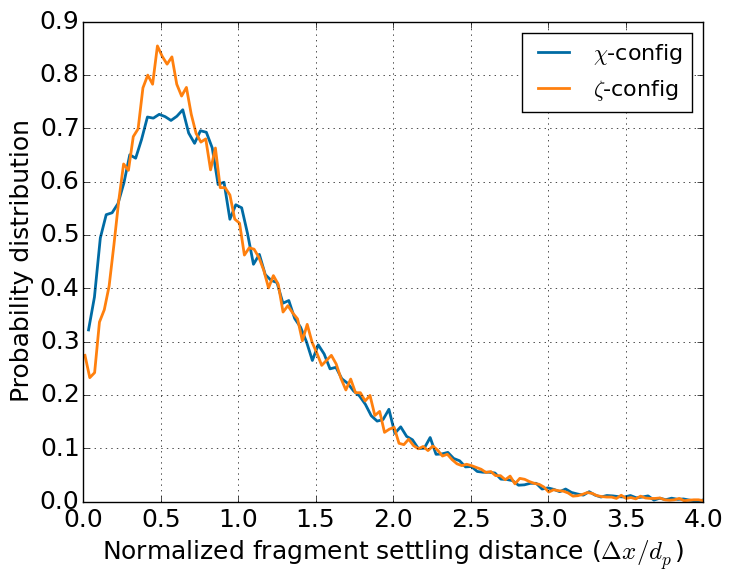
\includegraphics[width = 0.65\textwidth]{figures/displacement_histograms.png}
    \caption{Normalized displacement histograms for fragment sizes of $r_2^* = 0.2$ with $\eta = 5\%$. $\chi$-config: 59.7\% of fragments travel up to \SI{1}{\milli\meter} and 8.2\% travel more than \SI{2}{\milli\meter}; $\zeta$-config: 60.7\% of fragments travel up to \SI{1}{\milli\meter}, 7.9\% travel more than \SI{2}{\milli\meter}.}\label{fig:displacement_hists}
\end{figure}

% Conductive heat transport in granular materials is dependent on normal forces between pebbles, and normal forces need not be isotropically distributed through beds. To investigate directional dependence, we calculate angular distributions of granular contacts and forces between every pair of interacting pebbles in the ensemble. Contact angle is measured between vectors pointing between contacting pebbles and $\zeta$. In other words, the most direct path for heat out of the system is along contacts at angles of $\theta=0,\pi$; magnitudes of contact forces around those angles dictate the ability of systems to discharge heat to coolant. A mean contact force, $\langle F_n \rangle$, is found inside wedges of $\Delta\theta$ in the same manner described above for ensemble-averaged temperature values. Mean forces for varying fragmentation amount, fragmentation size, initial packing density, and orientation are plotted in \Cref{fig:force-polars}.
% , the stress tensor, $\mathbf{\sigma}$, is
% \begin{equation}
%   \sigma_{jk} = \frac{1}{V}\left(\sum_c d_0 f^{(n)} n_jn_k + \sum_c d_0 f^{(t)} n_jt_k\right)
% \end{equation}
% where $c$ indicates a contact pair of pebbles, $d_0$ is the separation distance between the centroids of the pebbles, $f^{(n)}$ and $f^{(t)}$ are the projected normal and tangential components of the contact force between the pair, and $\mathbf{n}$ and $\mathbf{t}$ are the normal and tangential unit vectors.
% \begin{figure*}[!tp]
%        \centering
%        \begin{subfigure}[b]{0.45\textwidth}
%                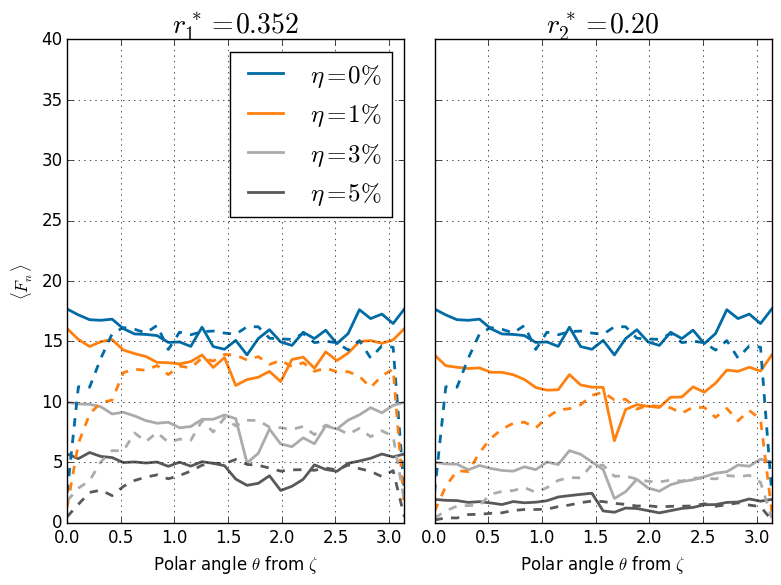
\includegraphics[width=\textwidth]{figures/62-percent-polar-forces.png}
%                \caption{Initial packing fraction of $\phi_1 = 0.62$.}
%                \label{fig:62-force-polar}
%        \end{subfigure}%
%        ~ %add desired spacing between images, e. g. ~, \quad, \qquad, \hfill etc.
%          %(or a blank line to force the subfigure onto a new line)
%        \begin{subfigure}[b]{0.45\textwidth}
%                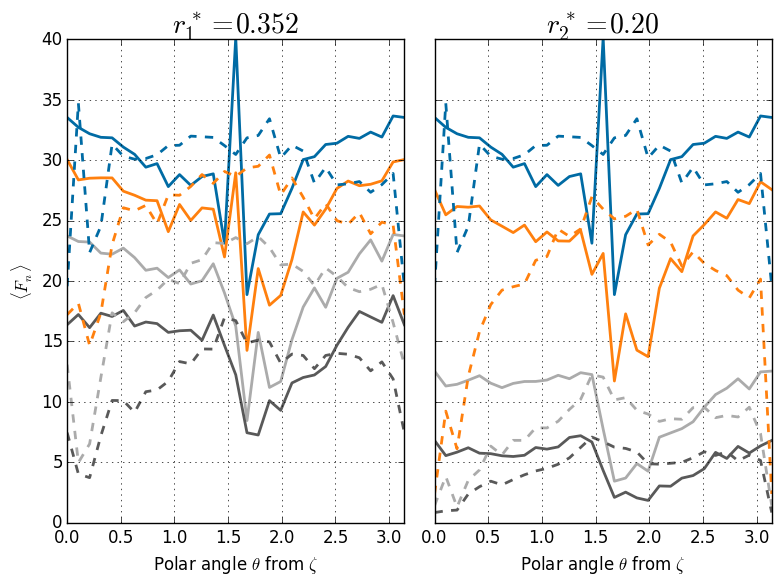
\includegraphics[width=\textwidth]{figures/64-percent-polar-forces.png}
%                \caption{Initial packing fraction of $\phi_2 = 0.64$.}
%                \label{fig:64-force-polar}
%        \end{subfigure}
%        \caption{Ensemble-average contact forces in wedges of angle $\Delta\theta$: solid lines are cases where gravity is in the $\chi$ direction ($\chi$-config), dashed lines for gravity in the $\zeta$ direction ($\zeta$-config); color is by percent of crushed pebbles.} %Grain orientation is such that polar angles of $\theta = 0,\pi$, are the directions of heat transfer in the bed.}
% \label{fig:force-polars}
% \end{figure*}

Analyzing results of all the pebble beds in this study revealed two main contributors to bed temperatures with resettling from pebble crushing: final settling location of fragment particles and overall contact force relaxation. The two interacting contributors were found to be expressed to different extents depending on crush amount and bed configuration.

Hydrostatic pressure (a global measure of inter-particle contact forces) is predominately a function of initial packing fraction alone, as seen in \Cref{fig:eta-sigma}. Smaller initial packing fractions had their internal hydrostatic pressures reduced more rapidly as pebbles crushed in the ensemble. Breeder orientation appears to have less impact on stress relief than size of crush fragments. Due to the inter-connected nature of the force network, and geometry of beds studied here, resettling in beds and contact force relaxation is uniform throughout the beds. Thus we expect reductions in contact forces to directly result in an overall increase of bed temperatures. This is reflected in the curves of \Cref{fig:eta-theta}. Total mean temperatures of $\phi_1 = 0.62$ beds increased between \numrange{16}{19}\% at $\eta = 5\%$. Yet beds initially packed to $\phi_2 = 0.64$ increased by only \numrange{10}{13}\% at the same value of crushed pebble amount.

Fragment settling location, on the contrary, is strongly dependent on fragment size and breeder orientation. Larger pebble fragments generally did not travel far, settling loosely in regions near the point of fragmentation. Smaller fragments were seen to be capable of traveling much further through interstitial gaps between pebbles before also coming to rest with loose settlings. The looseness of the fragment settling is indicated by their ensemble-average coordination number (counting only the fragments) for $r_1*$ and $r_2^*$, respectively, as $\langle Z \rangle = 3.2$ and $\langle Z \rangle = 2.8$. Contacts with walls or floors are not counted in this coordination number. A consequence of loose packings of fragments is poor thermal conductance to neighboring pebbles. Fragment temperatures are therefore mostly regulated by convection with interstitial helium and their influence on bed temperatures is much more complex.

To identify the effects of fragment settling, we look to \Cref{fig:displacement_hists} and the several zones demarcated in the results of \Cref{fig:1,fig:3}. The majority of fragments, even in this case of smallest fragment size and largest crushing amount, remain approximately at the location of the parent pebble; for both configurations, approximately 60\% travel less than 1 pebble diameter (\SI{1}{\milli\meter}). However, in both configurations, approximately 8\% of fragments travel more than 2 diameters, and those pebbles have a significant impact on the ensembles overall thermal response.

In $\zeta$-configuration beds, pebbles traveling more than a few pebble diameters will move between colored isotherms drawn in \Cref{fig:1}. For example we can see the fragment group identified in Zone (1) as moving downward, away from the top wall. Similarly, when pebbles in Zone (3) are crushed, some of the fragments tumble downward into Zone (2) before coming to rest where they continue to receive volumetric heating. Thus the fragments, with poor thermal conductance, increase heating in the regions where they settle. The effect is seen in the $\eta = 3, 5\%$ temperature profiles in \Cref{fig:64-T-profile} that are asymmetric with lower temperatures in the top half (above Zone (3)) and higher temperatures in the region near Zone (2).

In contrast, $\chi$-config beds respond much differently to pebble fragment settling. We again see from cross-sections in \Cref{fig:3} a pebble identified in Zone (1) that breaks but remains in that zone after settling. The trend continues in other regions of the bed. When pebbles are crushed in the $\chi$-config beds, gravity causes them to fall downward but remain generally in the same isotherm, as drawn in \Cref{fig:3}. According to \Cref{fig:64-T-profile}, the effect of pebble crushing has little effect up to 3\% of damaged pebbles. But suddenly at $\eta = 5\%$, the combination of reduced overall bed pressure and fragmentation heating causes the maximum bed temperature to jump above all other $\phi = 64\%$ beds (see \Cref{fig:64-T-profile} and \Cref{fig:eta-T_max}). The temperature increase in this $\chi$-config bed is due to the accumulation of pebble fragments that remain in Zone (3), only tumbling to lower heights. Helium that enters the $\chi$-configuration bed reaches higher temperatures more quickly due to the increased heating from fragments which settled at lower heights of $y$. Helium then continues to heat from the many fragments in Zone (3) which ultimately results in the highest maximum bed temperatures (for the given packing fraction). This can also be seen with comparison between \Cref{fig:1,fig:3}: the $\chi$-config bed reaches the \SI{780}{\kelvin} contour at a much lower height than the $\zeta$-configuration. 

Travel of pebble fragments also manifests in changes to local packing fraction. In \Cref{fig:x-62-r23-deltas,fig:x-62-r125-deltas,fig:x-64-r23-deltas,fig:x-64-r125-deltas}, we see the changes local packing fraction distribution, for all pebble beds of $\chi$-configuration, due to fragmentation and resettling. Similarly, in \Cref{fig:z-62-r23-deltas,fig:z-62-r125-deltas,fig:z-64-r23-deltas,fig:z-64-r125-deltas}, we see the local packing fraction distributions for all pebble beds of the $\zeta$-configuration. These figures are alternative depictions of fragmentation travel, illustrating global changes to pebble beds after pebble crushing. The images are generated from binning particles in grids of $x$ and $z$ and considering all pebbles in the depth $y$.

Comparing \Cref{fig:x-62-r23-deltas} with \Cref{fig:x-64-r23-deltas}, two sets of beds with the same configuration and fragment size but different initial packing fraction, we see pebble beds with lower initial packing fractions have an amplified response to crushing than beds with higher packing fraction. Likewise, if we flip the orientation such as in \Cref{fig:z-62-r23-deltas} and \Cref{fig:z-64-r23-deltas}, there is again a more widespread change in local packing fraction for beds of smaller initial packing fractions.

The effect of pebble fragment size to local packing fraction is also revealed in these images. For both configurations, and all initial packing fractions, the beds with smaller fragment size, $r_2^*$, would result in accumulation of mass (\textit{i.e.} higher packing fraction) at the base of the pebble beds and a reduction of mass near the top wall. Among this subset of pebble beds with smaller fragments, we again clearly see that lower initial packing fractions; beds of either configuration with $\phi = 0.62$ have larger regions of $\Delta \phi = 0.07$ than any of the $\phi = 0.64$ beds.
% \begin{figure}[!t]
%     \centering
%     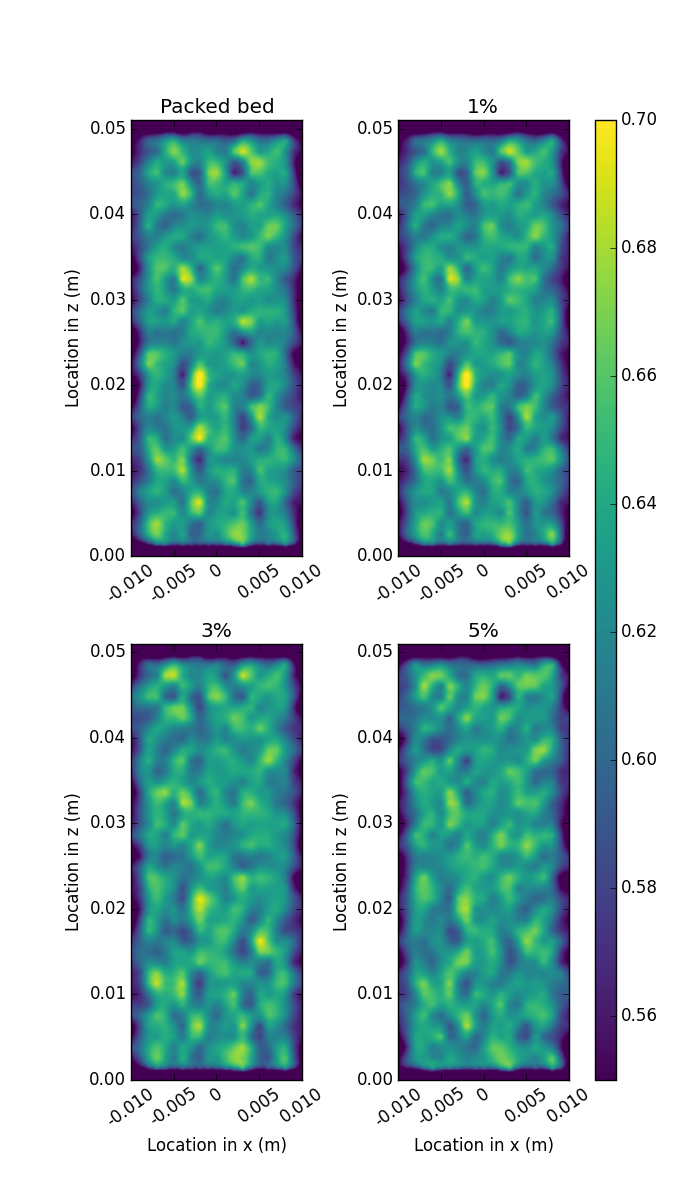
\includegraphics[width = 0.65\textwidth]{figures/x-62-r23-1.png}
%     \caption{Distribution of local packing fraction for $\chi$-config, $\phi = 0.62$, $r^* = 0.32$}\label{fig:x-62-r23}
% \end{figure}

% \begin{figure}[!t]
%     \centering
%     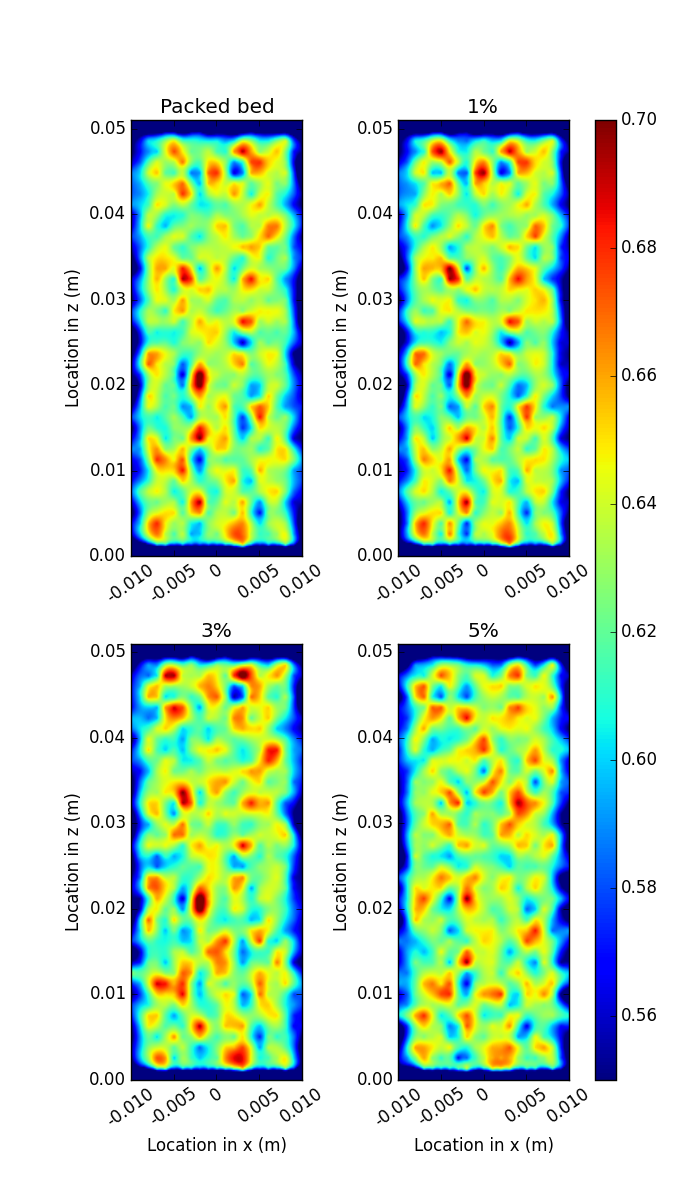
\includegraphics[width = 0.65\textwidth]{figures/x-62-r125-1.png}
%     \caption{Distribution of local packing fraction for $\chi$-config, $\phi = 0.62$, $r^* = 0.2$}\label{fig:x-62-r125}
% \end{figure}

% \begin{figure}[!t]
%     \centering
%     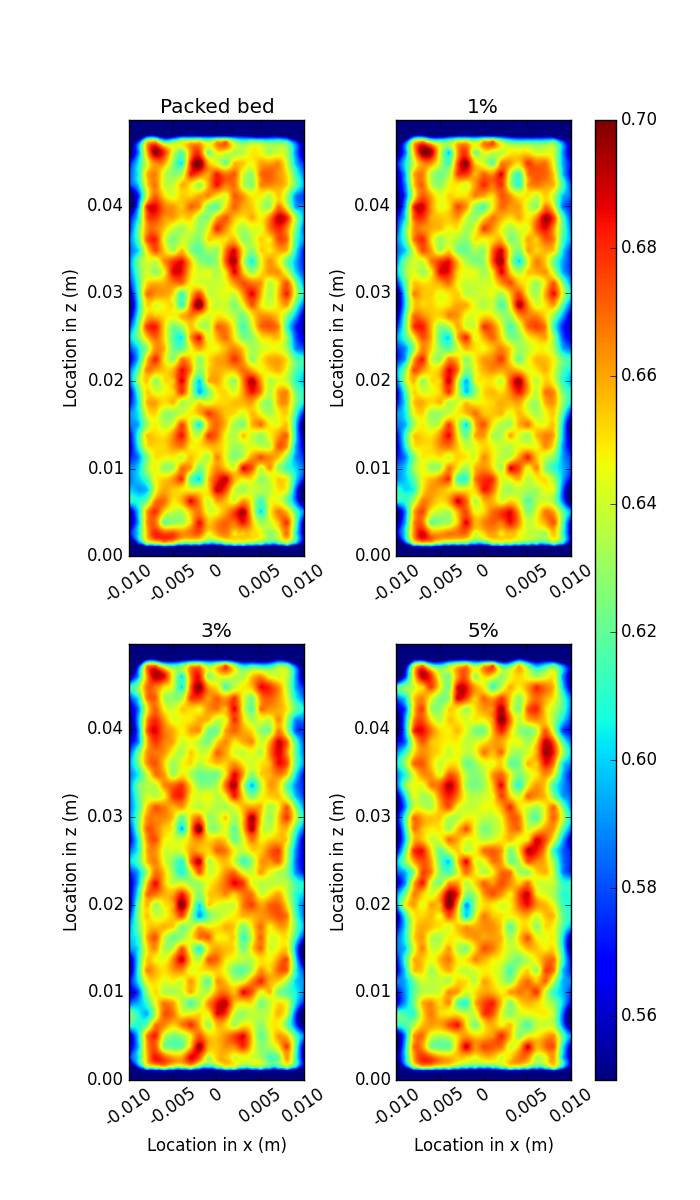
\includegraphics[width = 0.65\textwidth]{figures/x-64-r23-1.png}
%     \caption{Distribution of local packing fraction for $\chi$-config, $\phi = 0.64$, $r^* = 0.32$}\label{fig:x-624-r23}
% \end{figure}
% \begin{figure}[!t]
%     \centering
%     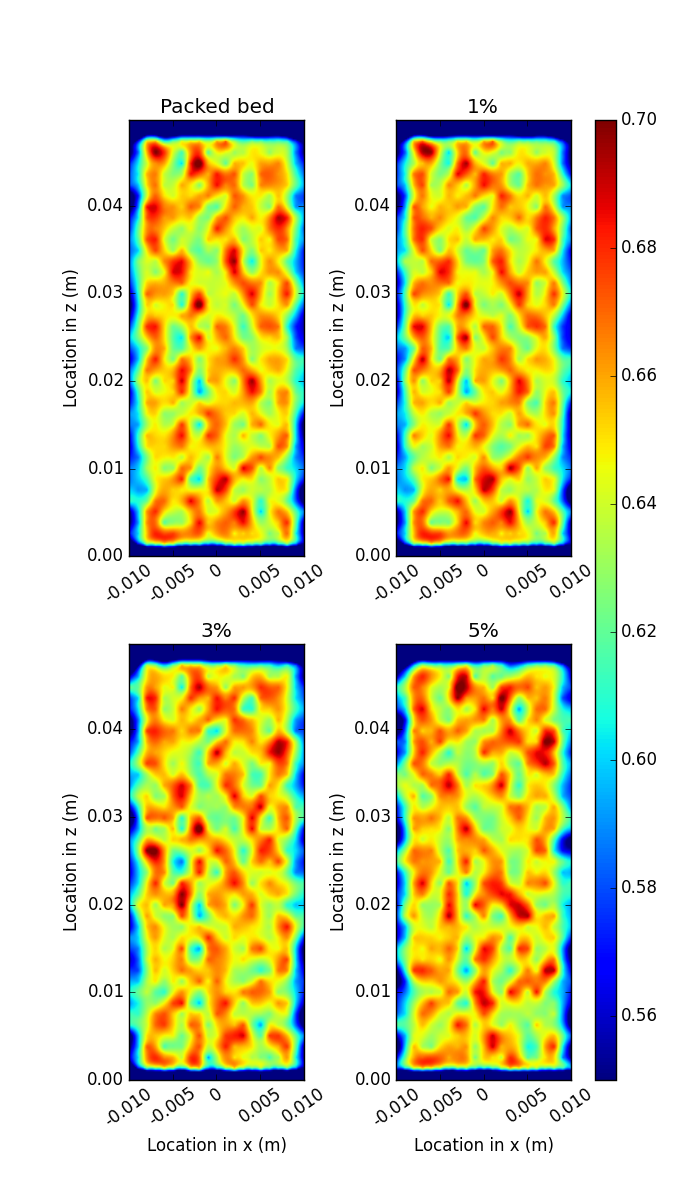
\includegraphics[width = 0.65\textwidth]{figures/x-64-r125-1.png}
%     \caption{Distribution of local packing fraction for $\chi$-config, $\phi = 0.64$, $r^* = 0.2$}\label{fig:x-624r125}
% \end{figure}


% deltas~~~~~~~~~~~~~~~~~~~~~~~~~~
\begin{figure}[!t]
    \centering
    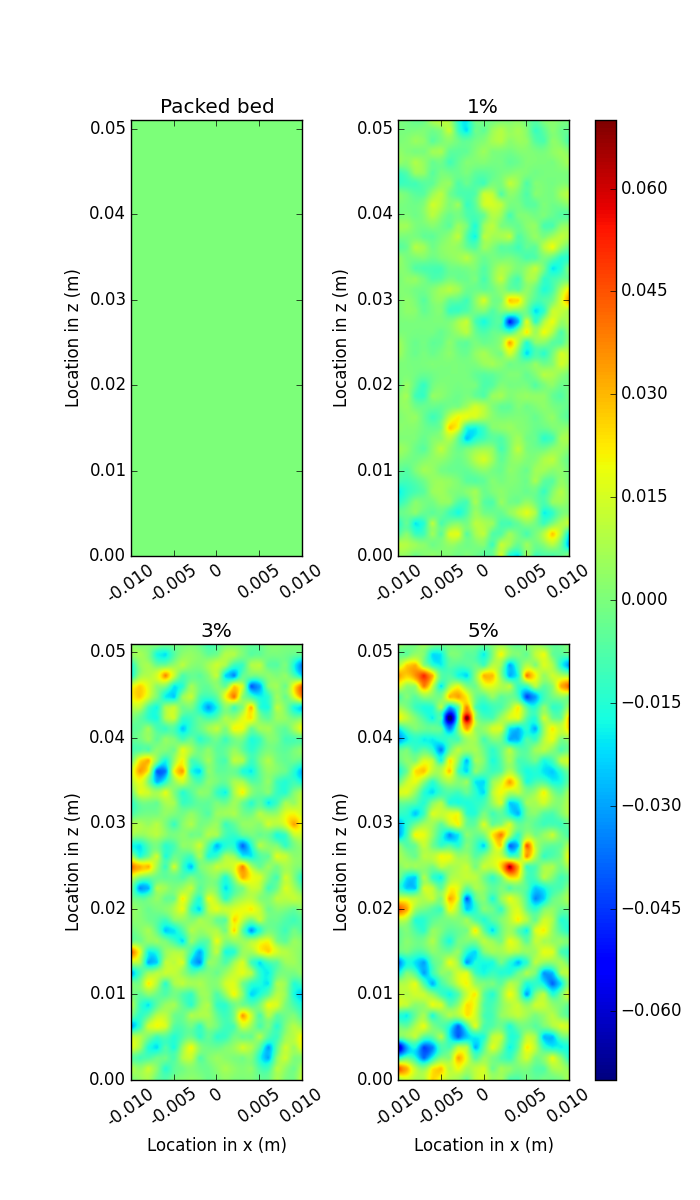
\includegraphics[width = 0.65\textwidth]{figures/x-62-r23-1-deltas.png}
    \caption{Distribution of local changes in packing fraction ($\phi_{\eta} - \phi_i$) for $\chi$-config, $\phi = 0.62$, $r^* = 0.32$}\label{fig:x-62-r23-deltas}
\end{figure}

\begin{figure}[!t]
    \centering
    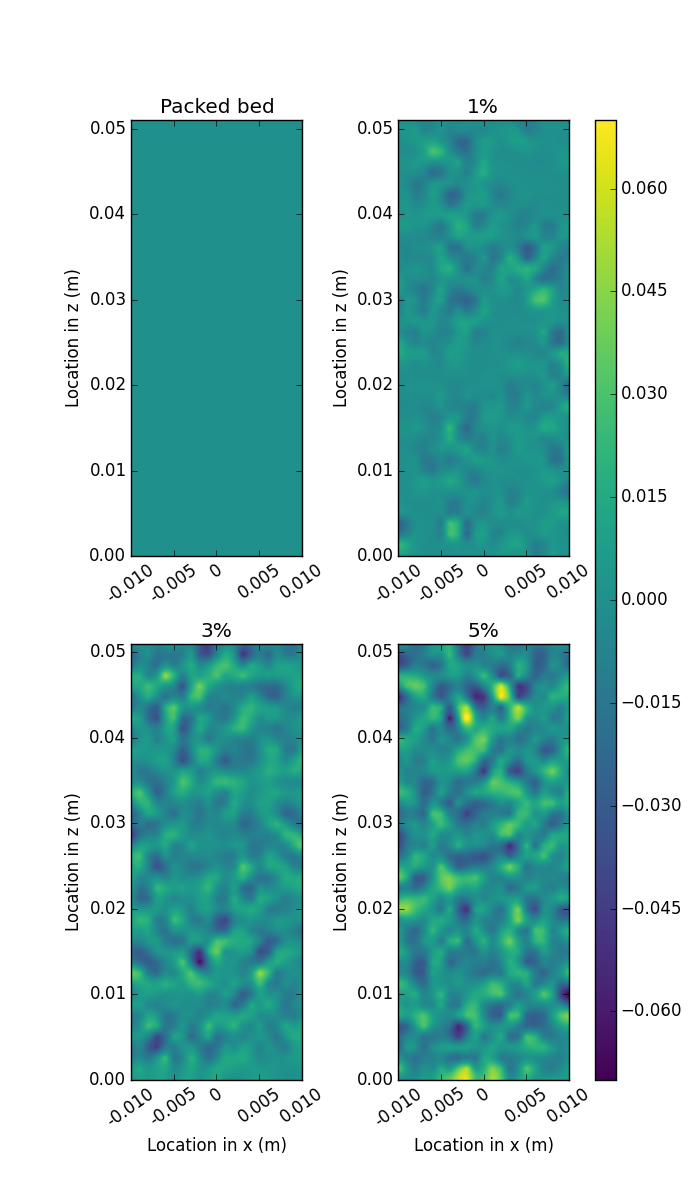
\includegraphics[width = 0.65\textwidth]{figures/x-62-r125-1-deltas.png}
    \caption{Distribution of local changes in packing fraction ($\phi_{\eta} - \phi_i$) for $\chi$-config, $\phi = 0.62$, $r^* = 0.2$}\label{fig:x-62-r125-deltas}
\end{figure}

\begin{figure}[!t]
    \centering
    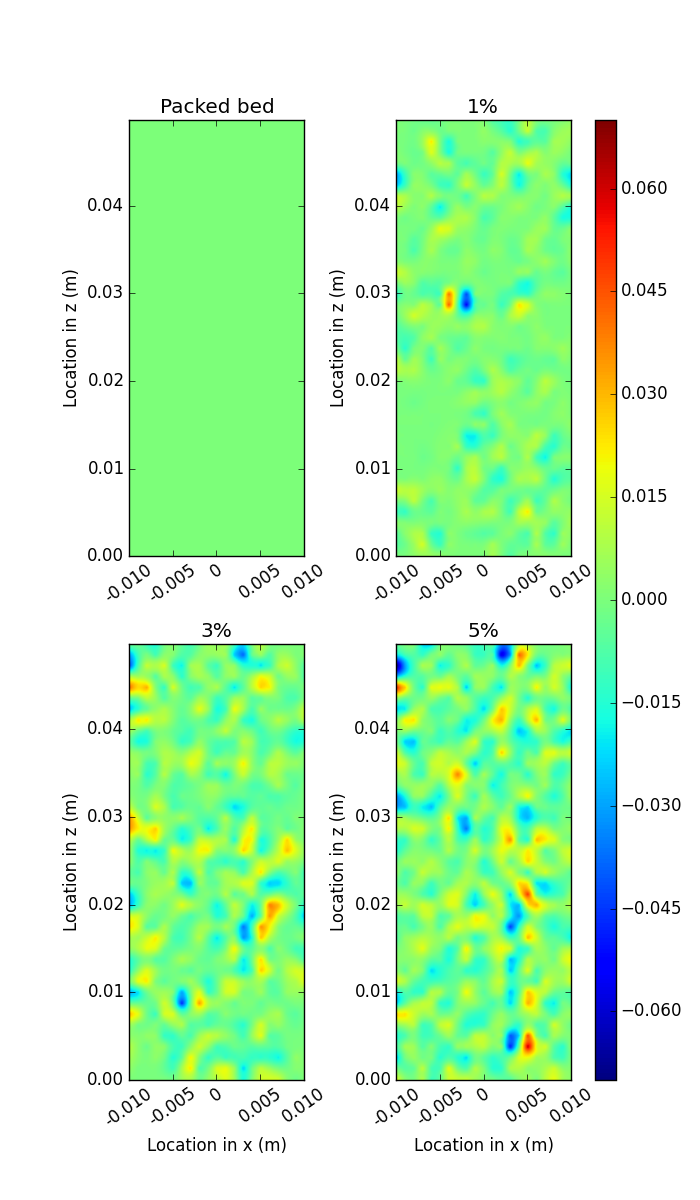
\includegraphics[width = 0.65\textwidth]{figures/x-64-r23-1-deltas.png}
    \caption{Distribution of local changes in packing fraction ($\phi_{\eta} - \phi_i$) for $\chi$-config, $\phi = 0.64$, $r^* = 0.32$}\label{fig:x-64-r23-deltas}
\end{figure}

\begin{figure}[!t]
    \centering
    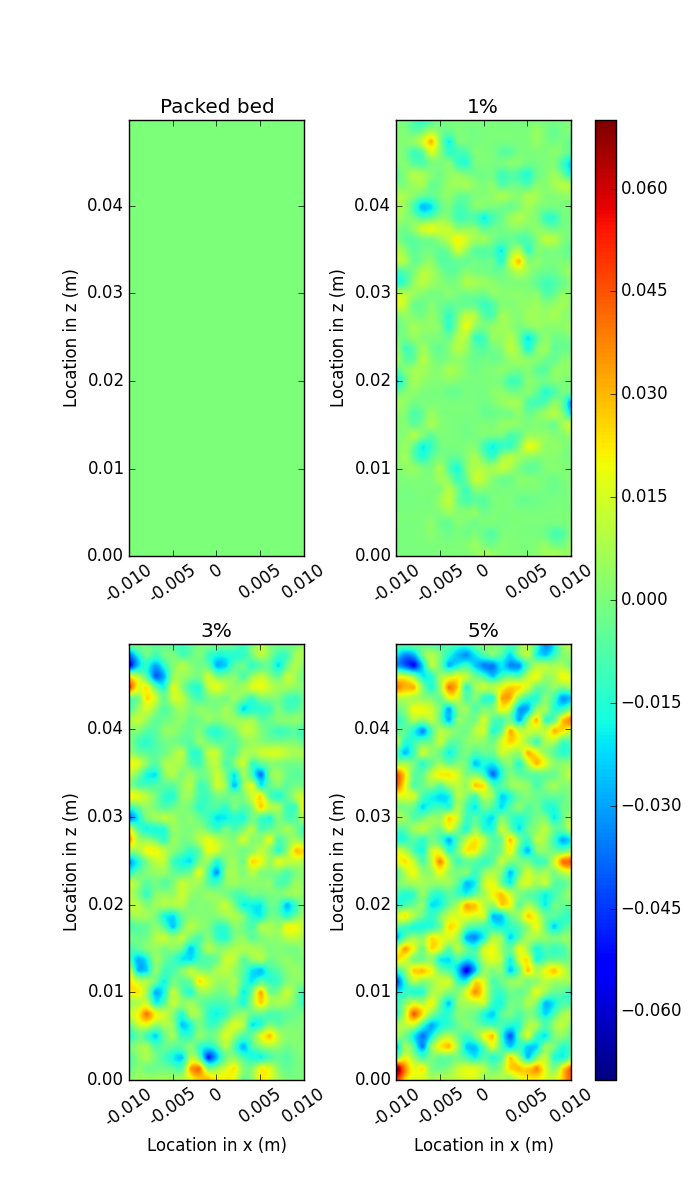
\includegraphics[width = 0.65\textwidth]{figures/x-64-r125-1-deltas.png}
    \caption{Distribution of local changes in packing fraction ($\phi_{\eta} - \phi_i$) for $\chi$-config, $\phi = 0.64$, $r^* = 0.2$}\label{fig:x-64-r125-deltas}
\end{figure}
% deltas~~~~~~~~~~~~~~~~~~~~~~~~~~



% \begin{figure}[!t]
%     \centering
%     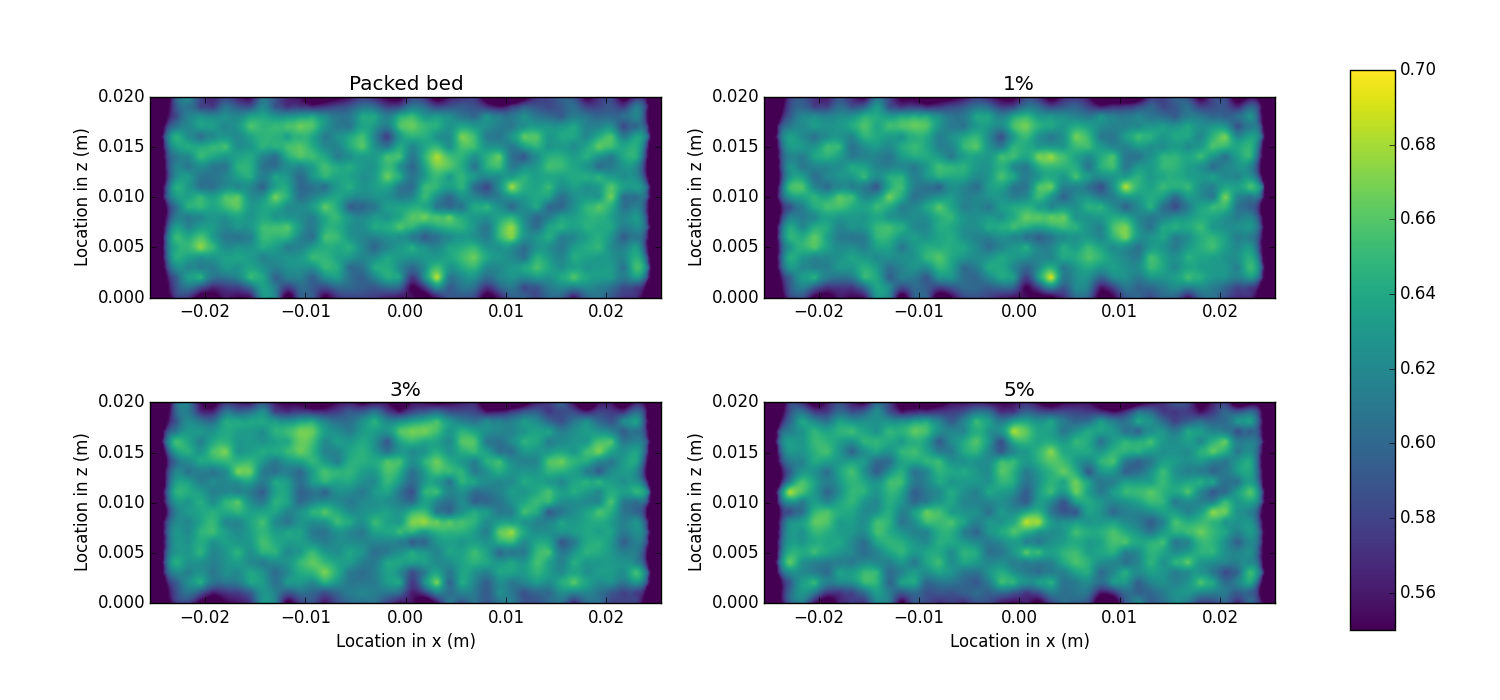
\includegraphics[width = 0.95\textwidth]{figures/z-62-r23-1.png}
%     \caption{Distribution of local packing fraction for $\zeta$-config, $\phi = 0.62$, $r^* = 0.32$}\label{fig:z-62-r23}
% \end{figure}
% \begin{figure}[!t]
%     \centering
%     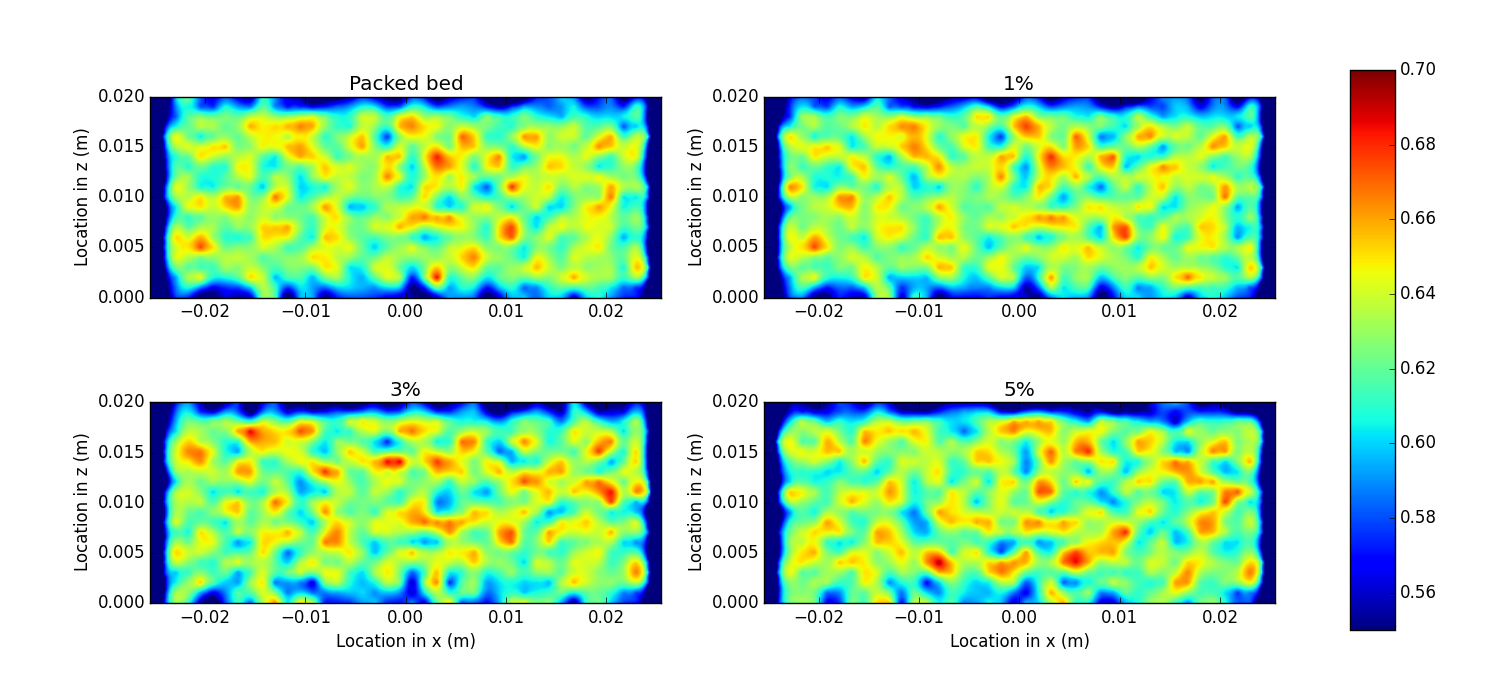
\includegraphics[width = 0.95\textwidth]{figures/z-62-r125-1.png}
%     \caption{Distribution of local packing fraction for $\zeta$-config, $\phi = 0.62$, $r^* = 0.2$}\label{fig:z-62-r125}
% \end{figure}
% \begin{figure}[!t]
%     \centering
%     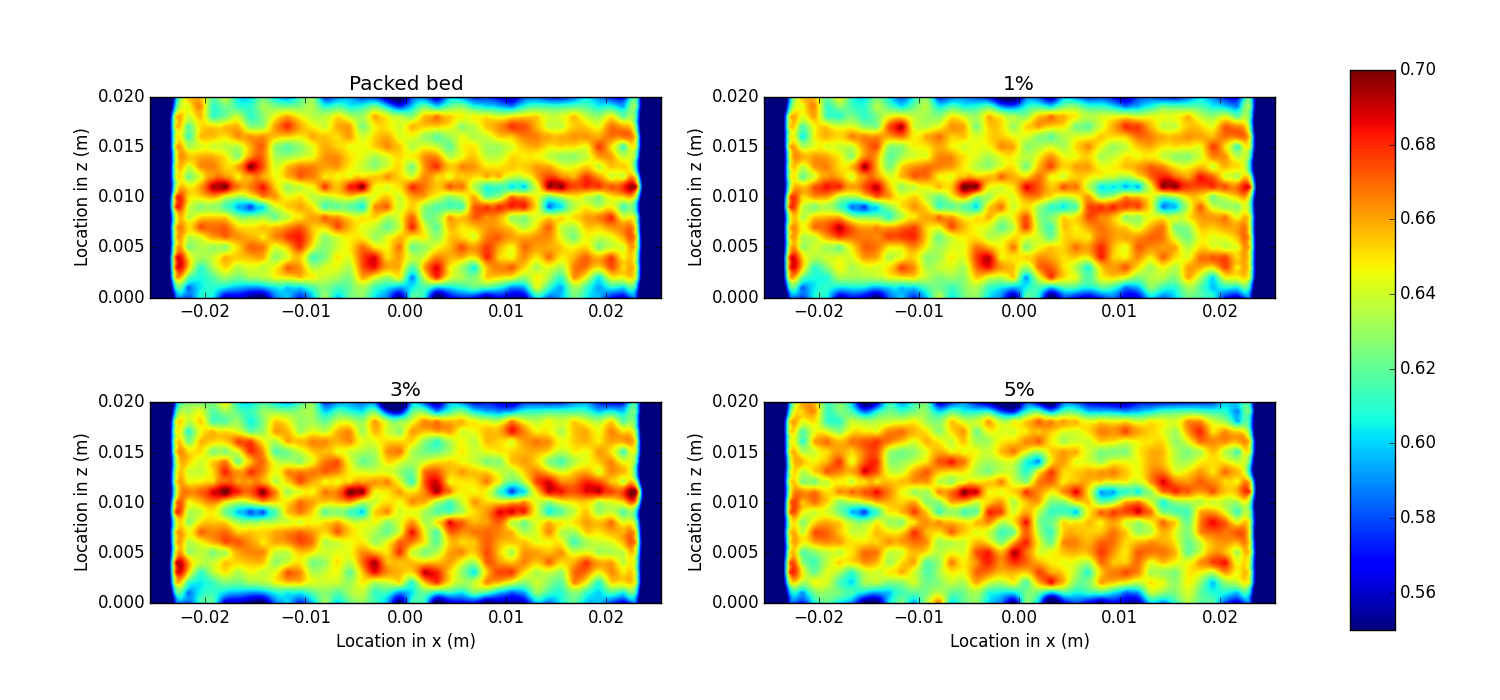
\includegraphics[width = 0.95\textwidth]{figures/z-64-r23-1.png}
%     \caption{Distribution of local packing fraction for $\zeta$-config, $\phi = 0.64$, $r^* = 0.32$}\label{fig:z-624-r23}
% \end{figure}
% \begin{figure}[!t]
%     \centering
%     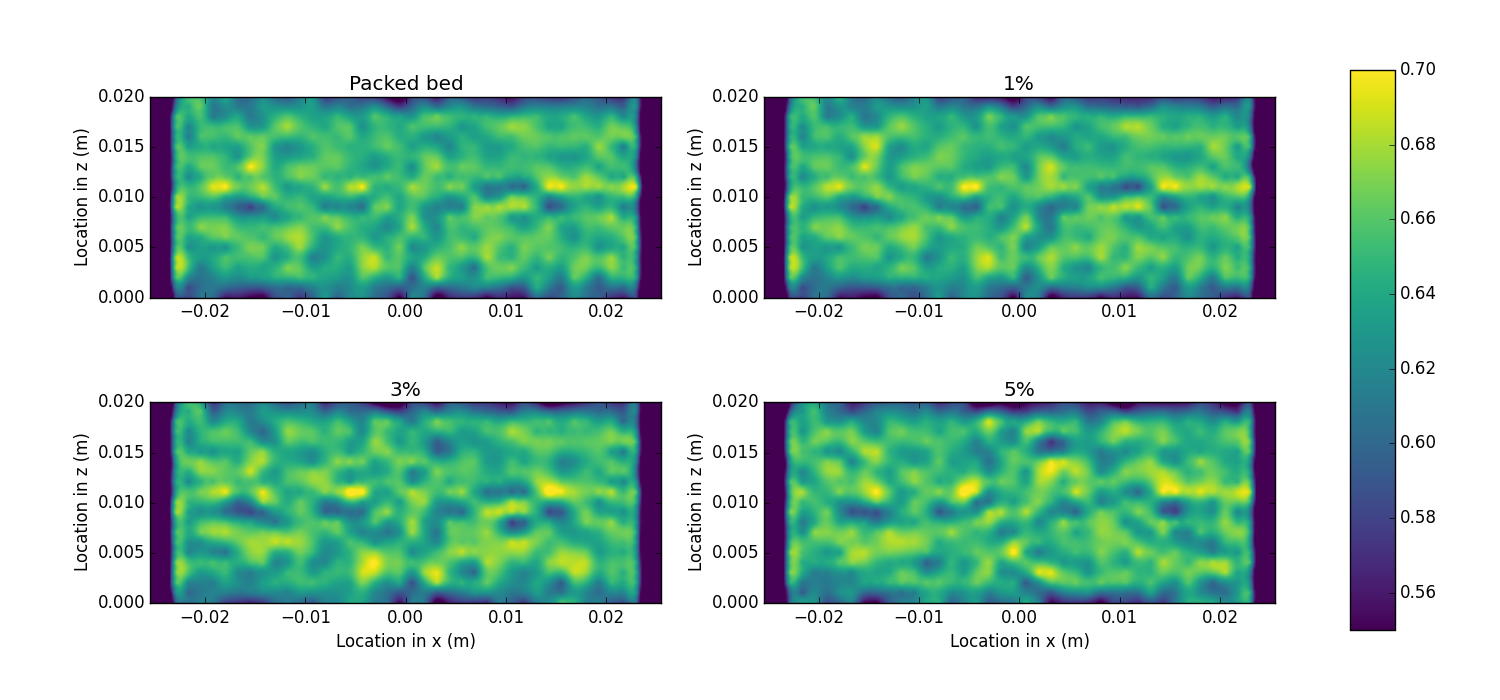
\includegraphics[width = 0.95\textwidth]{figures/z-64-r125-1.png}
%     \caption{Distribution of local packing fraction for $\zeta$-config, $\phi = 0.64$, $r^* = 0.2$}\label{fig:z-624r125}
% \end{figure}



% deltas~~~~~~~~~~~~~~~~~~~~~~~~~~
\begin{figure}[!t]
    \centering
    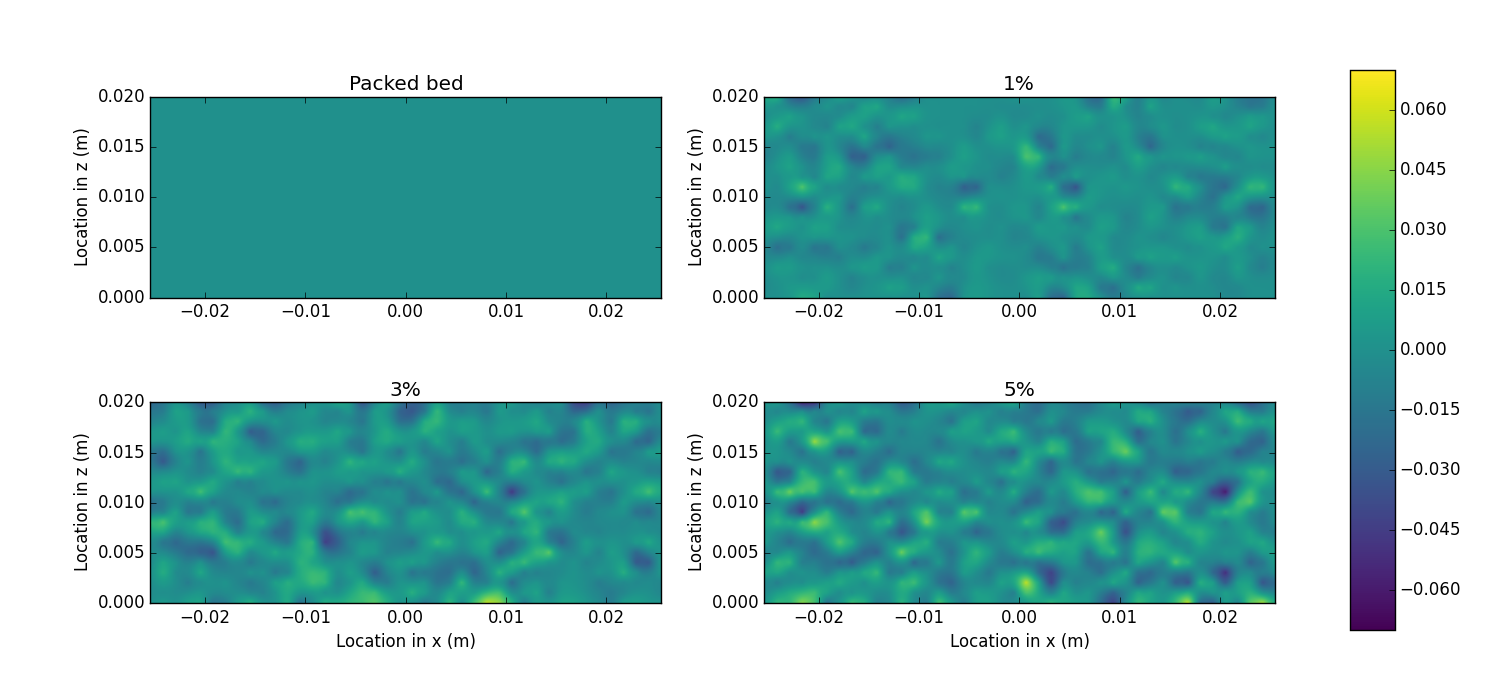
\includegraphics[width = 0.95\textwidth]{figures/z-62-r23-1-deltas.png}
    \caption{Distribution of local changes in packing fraction ($\phi_{\eta} - \phi_i$) for $\zeta$-config, $\phi = 0.62$, $r^* = 0.32$}\label{fig:z-62-r23-deltas}
\end{figure}

\begin{figure}[!t]
    \centering
    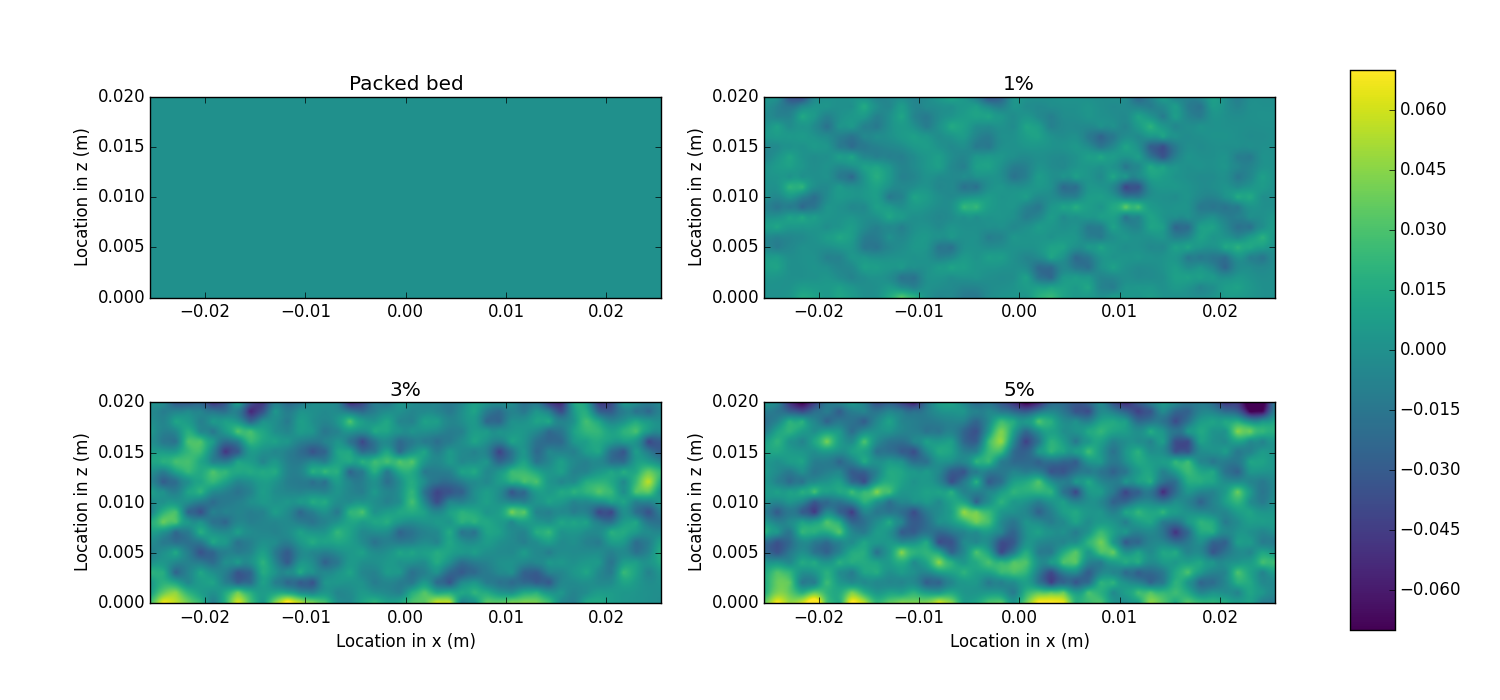
\includegraphics[width = 0.95\textwidth]{figures/z-62-r125-1-deltas.png}
    \caption{Distribution of local changes in packing fraction ($\phi_{\eta} - \phi_i$) for $\zeta$-config, $\phi = 0.62$, $r^* = 0.2$}\label{fig:z-62-r125-deltas}
\end{figure}

\begin{figure}[!t]
    \centering
    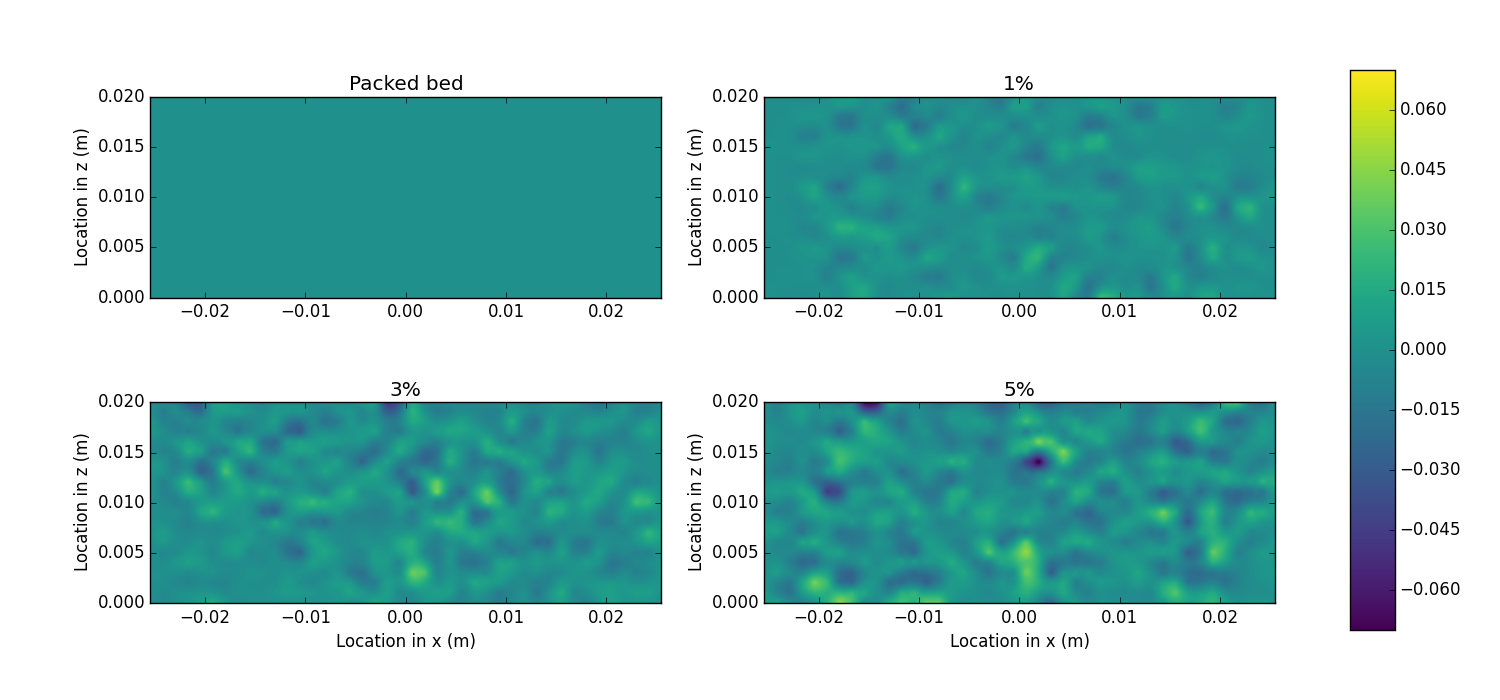
\includegraphics[width = 0.95\textwidth]{figures/z-64-r23-1-deltas.png}
    \caption{Distribution of local changes in packing fraction ($\phi_{\eta} - \phi_i$) for $\zeta$-config, $\phi = 0.64$, $r^* = 0.32$}\label{fig:z-64-r23-deltas}
\end{figure}

\begin{figure}[!t]
    \centering
    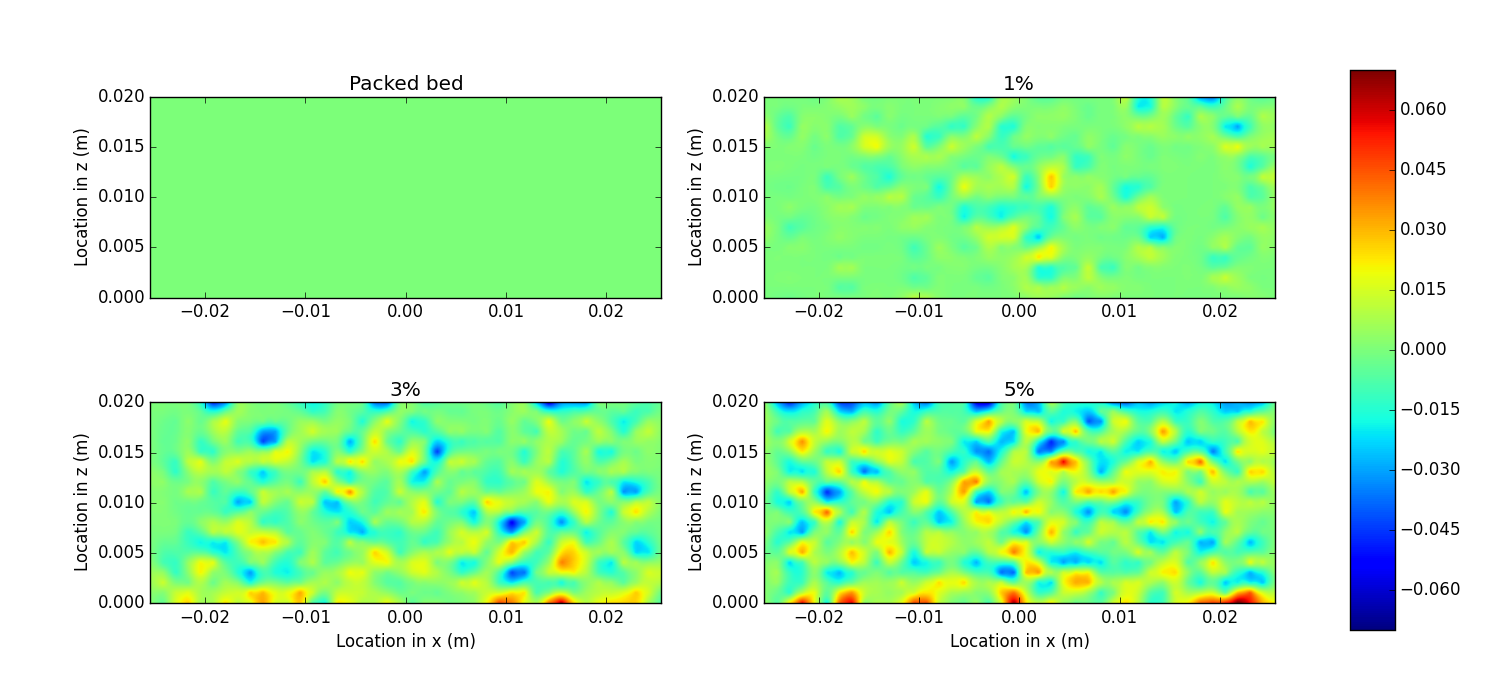
\includegraphics[width = 0.95\textwidth]{figures/z-64-r125-1-deltas.png}
    \caption{Distribution of local changes in packing fraction ($\phi_{\eta} - \phi_i$) for $\zeta$-config, $\phi = 0.64$, $r^* = 0.2$}\label{fig:z-64-r125-deltas}
\end{figure}
% deltas~~~~~~~~~~~~~~~~~~~~~~~~~~


\FloatBarrier

%in each configuration is the near-wall region where pebbles contact walls. In $\chi$-config bed in \Cref{fig:3}, we can see how pebble fragments tumble downward but generally remain in the near-wall region of Zone (1). Conversely, we see clearly in the $\zeta$-config bed of \Cref{fig:1} that some fragment groups leave the region and resettle downward toward the bed's central region. The differences in settling between the two configurations is consistent when we consider pebble behavior in other zones.

%Zones (2) are the moderate temperature regions of \Cref{fig:1,fig:3}, the approximate location is also shown on temperature profiles in \Cref{fig:64-T-profile}. For $\zeta$-configs, temperatures shown in \Cref{fig:64-T-profile} demonstrate an asymmetric lump in profile that is absent in $\chi$-config beds. Increases in Zone (2) temperatures for $\zeta$-config beds are due to the fraction of pebbles which freely tumble through interstitial gaps, influenced by gravity, into Zone (2) from other regions. Once settled, the increased masses of ceramic in Zone (2) then create additional heating from the volumetric source. It should be noted that the exact location of the `lumps' in temperature profiles measured here are unique to the pebble bed considered in this study and the random location at which the fragments accumulated, however the phenomena of increased temperature in the lower-half of $y$-locations of beds with crushed pebbles will consistently appear. As for the $\chi$-configurations, pebbles broken in Zone (2) see their daughter fragments remain in Zone (2) as they tumble in the $y$-direction, regardless of the distance. No added mass in the region results in no abnormal increases in Zone (2) temperature profiles; only overall increases of temperatures are witnessed. 

%For $\zeta$-config beds, a similar effect of fragment-travel into and out of Zone (3) occurs, long-distance traveling of the roughly 10\% of pebbles in $\zeta$ configuration contributes to spreading heat generation from the high temperature regions into regions at lower heights of $y$. However, in $\chi$-config beds, pebbles that crush in Zone (3) again have fragments which generally remain in Zone (3) regardless of distance traveled. The accumulating pebble fragments in Zone (3) continue to receive nuclear heating but have very poor contact conductance with neighboring pebbles. The flowing helium purge gas prevents runaway high temperatures of these fragments but the end results are higher maximum temperatures. In the case of $r_2^*$ at $\eta = 5\%$, we see in \Cref{fig:eta-T_max} the maximum temperatures in $\chi$-config beds overtake the maximum temperatures of similar $\zeta$-config beds. This large increase in maximum temperature rise is due entirely to small fragments accumulation in Zone (3), the similar bed of $\zeta$-configuration shows a much lower maximum bed temperature rise. It is also interesting to note the two beds with smallest temperature rise among any studied here were $\zeta$-configurations. Yet at the same time, those two beds saw similar or more increase in overall bed temperatures in comparison to $\chi$-configurations. These results demonstrate the effect of pebble fragments traveling between zones in $\zeta$-config beds: increasing temperatures in moderate-temperature zones with a trade-off of decreased temperatures in high-temperature zones.

%Looking to \Cref{fig:eta-T_max}, among all the solid lines ($\phi_2 = 0.64$) we see a large jump in bed temperature rise only for the $\chi$-config bed at $\eta = 5\%$ with $r_2^*$; the maximum bed temperature even jumps above most of the less-tightly packed $\phi_1$ beds. It is interesting to note that a similar set of parameters ($\phi_2, r_2^*, \eta_5$) in the $\zeta$-configuration shows a much lower maximum bed temperature rise. Furthermore, 

%, the phenomena of inter-granular resettling strongly impacting temperature rises only occurred for beds with small fragmentation sizes, $r_2^* = 0.2$; see $(\phi_2, \chi_g, r_w^*)$ at $\eta = 5\%$. This is attributed to the tightly packed structures of these well-packed beds. But when the initial packing fraction was reduced, $\phi_1$, for instance, increases in maximum temperatures due to fragment resettling was seen even for larger fragments, $r_1^* =  0.52$. 

%Results shown here illustrate many unique features of heat transfer in granular materials with crushed pebbles and fluid flow. 
%From the temperature profiles of \Cref{fig:T-profiles}, smooth parabolic temperature profiles for initially-packed beds ($\eta = 0$ for both $\phi_{1,2}$) indicate constant $\keff$ values and support the use of continuum theory for those granular assemblies. However, for $\eta > 0$, at all packing fractions and fragmentation radius ratios, temperature profiles become increasingly jagged with large jumps in mean temperatures along $\zeta$ due to heating of crush fragments and distribution of contact forces. Standard models with continuum treatment of granular material cannot predict this manner of inhomogeneous transport of heat in pebble beds. The $\keff$ model must be re-evaluated for use with crushable granular materials.

%for larger crush fragments ($r_1^*$), temperature profiles remained near-perfect parabolas, indicating constant $\keff$ and rough applicability of continuum, for all initial packing fractions and granular crush amounts. However, when fragments were smaller ($r_2^*$), the profiles became more jagged deviation began to occur as crush amount increased. The importance of the profile is in its indication of a constant $\keff$ through the granular material; from the boundary conditions of the system, the more constant the $\keff$, the more perfectly parabolic the temperature profile. This has important repercussions on the the $\keff$ treatment of the granular ceramic as a continuum medium in macro-scale simulations. 

%In \Cref{fig:eta-theta}, total mean temperatures as functions of granular crushing amount are given. Some observable trends: 1) lower initial packing fractions, \textit{i.e.} $\phi_1$, see greater reductions in bed stress and greater mean bed temperatures as pebbles are crushed ; 2) beds with with heat outflow in the direction of gravity ($\zeta$-config) generally had higher bed temperatures for all granular crushing amounts compared to beds with heat outflow perpendicular to gravity ($\chi$-config); 3) size of granular fragment had little impact on bed stresses (until $\eta = 5\%$), but generally beds with smaller fragments had higher temperatures due to small fragments having very small conductive heat transport; 4) when considering fragmentation, there is a weak relationship of internal stress to mean bed temperature. For example, comparing cases of $\phi_2$, $\chi_g$ with the two $r^*_{1,2}$ as functions of $\eta$. For $\eta = 0, 1, 3\%$, stress falls to almost identical values (\Cref{fig:eta-sigma}), yet temperatures for the bed with $r_2^*$ have much higher mean temperatures for all fragmentation amounts.
%If one were to rely only on indirect measurements of pebble bed integrity, \textit{i.e.} measurements of bed pressure load, changes to pebble bed temperature might go unnoticed.

%The polar angle, $\theta$, shown from $0$ to $\pi$ in \Cref{fig:force-polars} is always measured as the angle from $\zeta$ direction -- the mean direction for heat transport to coolant. Thus for all cases, the angles near $\theta = 0,\pi$ correspond to pebbles contacting and transferring heat towards the coolant. Whereas contact between pebbles at angles near $\theta = \pi/2$ correspond to contacts approximately along isotherms in $\chi$ directions (see \Cref{fig:62xpebs}) with little impact on bed heat removal. These plots are more indicative of a pebble bed's ability to transport heat to coolant than bed stresses in \Cref{fig:eta-sigma}. Configurations with $\chi$-direction gravity see higher contact forces near $\theta = 0, \pi$ for all parameters, compared to similar $\zeta$-config beds; likewise the temperatures of $\chi$-config beds are always cooler than similar $\zeta$-config beds. 
%For $\chi$-config cases of \Cref{fig:62-force-polar,fig:64-force-polar}, forces near $\theta = 0,\pi$ are reduced less as individual pebbles are crushed in the ensemble than comparable $\zeta$-config cases. For example, for $\phi_2$, $r^*_1$, mean contact forces near $\theta=0,\pi$ drop by approximately 51\% for $\chi$-configurations whereas mean normal forces drop by nearly 65\% for $\zeta$-configurations. 
%When the internal stress is calculated for pebble beds (for \Cref{fig:eta-sigma}), directional dependence of contact forces is ignored; large forces near $\theta = \pi/2$ mask the reductions in contact forces along heat removal routes. %Therefore overall internal stress of a bed may not drop by a large degree due to large contact forces near $\theta = \pi/2$ directions, but heat transport to boundaries may be strongly affected and temperatures will rise in the bed. 
%This phenomena was observed and mentioned in discussions of \Cref{fig:eta-plots}; and is explainable by directional-dependencies of contact forces and heat transfer in granular systems.


\subsection{Conclusions}
We conducted several microscale simulations of granular heat transfer using coupled CFD-DEM simulations of representative tritium-breeding ceramic pebble bed volumes with parametric variations of: bed orientation with respect to gravity, pebble crushing amount, initial packing fraction, and crushed fragmentation size.

There was one general trend observed that reiterates past conclusions from solid breeder research. Namely, more persistent behavior is witnessed in pebble beds with higher initial packing fractions. In this study, the most dominant parameter observed to affect temperatures in pebble beds was the initial packing fraction: beds with higher initial packing fraction had smaller increases in bed temperatures due to pebble crushing. We therefore conclude that manual densification, from either long-term vibration packing or load-induced pre-compaction, must be done to ceramic pebble bed volumes to gain some temperature control during operation in a fusion reactor. To achieve packing fractions of $64\%$ in the relatively small sizes of this study, for example, a load of over \SI{1}{\mega\pascal} was necessary. In the assembly of tritium breeding modules, it must be kept in mind that similar pre-compaction may need to be performed.

As stated earlier, a concern with the $\zeta$ design is the possibility of gap formation between pebble bed and upper walls after bed resettling, particularly after pebble fragmentation. In this study, we found pebble beds initially packed to $\phi = 62\%$ experienced the highest increases in both total average bed temperature as well as maximum temperature rise. The comparably looser packing allowed a quick reduction in hydrostatic pressures and consequently a reduction in heat conduction to the upper wall. Nevertheless, no gaps were detected even at 5\% of pebbles crushed. However, temperatures in pebble beds packed to 64\% showed a resistance to fragmentation; overall average temperatures were comparable to $\chi$-configurations, and in fact these EU-style beds had the lowest maximum temperatures for beds with many crushed pebbles. We showed that freedom of fragments to travel between zones in these beds prevented a build-up of loose fragments (and thereby avoided build-up of heating) in the hottest regions.

As for the $\chi$-configurations, we found that when there were not many broken pebbles ($\eta \le 3$\%), these beds generally had lower temperatures in comparison to similar $\zeta$-config beds. But as $\eta$ went above 3\% for many of the beds, the averaged bed temperature and, importantly, the maximum temperature rise actually jumped above the $\zeta$-configurations. We showed that for these beds it was the inability for fragments to move between zones which left many small fragments to settle in the hottest region, further contributing to heating.

From the results we have shown, it is obvious that pebble crushing and bed resettling effects on temperature are complicated, non-linear responses and are particular to breeder design and ceramic material employed. We found indications of certain operational spaces for which different designs responded less severely to pebble crushing. For instance, from the point of view of temperature response in pebble beds, if one were to employ a material known to have a limited crush strength, one might accept that many pebbles could break (at least up to 5\%, as studied here) over the life of the breeder and choose to employ the $\zeta$-style which avoided large increases in temperature after long operation of the breeder. Alternatively, if one had a ceramic material with a larger crush strength, the $\chi$-design would be preferable as it generally retained lower overall and maximum bed temperatures when fewer pebbles in the ensemble were crushed.

It must be pointed out that the findings discussed here are concerned primarily with temperature distribution, without consideration for other consequences of pebble crushing such as blocking of helium purge, and thereby tritium extraction, by clogging from fragment dust or particulates. Clogging of purge flow is specific to each pebble bed design and must receive future attention in its own right.

This study was performed on some generic geometries and has provided some generalized conclusions. But in light of the pebble beds' complex responses, as breeder designs continue to evolve into their final form before deployment in ITER, CFD-DEM models should continuously be employed to study the specific thermomechanical responses to pebble crushing and bed resettling unique to each design.


%  We showed that granular crushing in an ensemble resulted in inhomogeneous contact force directional distributions. We also concluded that temperature distributions in beds with granular crushing are not predictable with $\keff$ approximations; demonstrating the limited applicability of continuum modeling of heat transfer in granular material without special consideration for evolving and time-dependent morphologies of the beds. We also discovered that, as pebbles crushed in an ensemble, the effects of structural orientation were reduced in beds with high initial packing fractions. Additionally we found that directional-dependencies of contact forces (\textit{i.e.} magnitudes of contact forces at specific angles of $\theta$) must be considered in situations where there is directional-dependence of heat outflow from bed to coolant.







\FloatBarrier
%%%%%%%%%%%%%%%%%%%%%%%%%%%%%%%%%%%%%%%%%%%%%%%%%%%%%%%%%%%%%%%%%%%%%%%%%%%%%%%%%%%%%%%%%%%%%%
\section{Lattice-Boltzmann Method Modeling of Temperature Distributions in Pebble Beds}\label{sec:lbm-studies}
%3D Lattice-Boltzmann Models of the Complete Conjugate Heat Transfer of Helium Purge Gas and Ceramic Pebble Beds
In this section, lattice-Boltzmann method (LBM) numerical models are used to study the complete interstitial flow of helium through a packed bed of lithium ceramics. A discussion on the development of the LBM method was given in \Cref{sec:modeling-lbm}. To review, for implementation of DEM and LBM coupling, pebble packing structures are generated with DEM simulations then mapped into the LBM nodal grids where the thermofluid and conjugate heat transfer models solve momentum and thermal conservation equations. The DEM-LBM approach is a one-way coupled approach in that LBM results are not currently fed back into DEM simulations for future packing evolution. The sacrifice of two-way coupling (that is currently possible with volume-averaged CFD-DEM models) offers instead to understand the tortuous helium flow and its impact on thermal transport in the tritium breeding ceramic pebble beds.

In the lattice-Boltzmann formulation, we will consider representative pebble bed volumes. The system spans $6d_p$ and $4d_p$ in the $x$ and $y$ directions, respectively. Primitive walls are placed at the limits of $x$, periodic boundary conditions are used in the extent of $y$. The limit in the flow direction, $z$, is set to satisfy the desired packing fraction of $\phi = 0.61$ with an ensemble of $N = 200$ pebble,
\begin{equation}
z_\text{lim} = \frac{N\pi d_p^3}{6x_\text{lim}y_\text{lim}\phi}
\end{equation}
where $x_\text{lim}$ and $y_\text{lim}$ are the limits given above. The result is approximately 7 pebble diameters of height ($7.16 d_p$) in the flow direction. Primitive walls are also placed at the limits of $z$.

The damaged pebble bed case considers fragments of size $r^* = 0.2$ and a damage amount of $\eta = 5\%$ (following the syntax developed in \Cref{sec:isfnt-12}). A resolution of $\res = 40$ is chosen in order to properly resolve the smaller fragments of the bed with damaged pebbles. Such a resolution dictates lattices of size $N_x = 241$, $N_y = 161$, and $N_z = 368$ for a total of approximately 14.2 million LBM nodes. The grid spacing is $\delta_x = \num{25e-3}$. A lattice velocity is chosen as $u_{0,lb} = 0.02$ which sets the lattice timestep size as $\delta_t = \num{500e-6}$. 

The relaxation parameters, $\omega$, for the lattice solving the momentum equation ($\omega_{ns}$), the lattice nodes representing the solid in the energy equation ($\omega_{cj}$) and the lattice nodes for the fluid in the energy equation ($\omega_{ad}$) are given in \Cref{tab:lbm-relaxations}.

The simulation procedure begins with creating volumes in DEM of a well-packed pebble bed and a pebble bed with crushed and fragmented particles. The two pebble beds are shown in their DEM representation in \Cref{fig:dem-for-lbm}. In order to highlight the differences between modeling methods, the pebble-fluid system will also be simulated in the CFD-DEM framework. 

% \begin {table}[ht] %
% \caption{Physical description of the lattice (in lattice units).}
% \label{tab:lbm-parameters} \centering %
% \begin {tabular}{ ccccc }
% \toprule %
% $N_x$   &   $N_y$  &   $N_z$    &   $\delta_x$   & $\delta_t$    \\\toprule
% 639      &   200     &   50     &    0.1         &  0.001        \\\bottomrule
% \end{tabular}
% \end{table}

\begin {table}[ht] %
\caption{The momentum relaxation constants for fluid (ns), thermal relaxation constants for fluid (ad), and thermal relaxation constants for the solid (cj) used in the simulation.}
\label{tab:lbm-relaxations} \centering %
\begin {tabular}{ cccccccc }
\toprule %
$\omega_{ns}$ &  $\omega_{ad}$  &   $\omega_{cj}$     \\\toprule
0.6569      &  0.3925       &   0.6995         \\\bottomrule
\end{tabular}
\end{table}

\begin{figure}[!ht]
    \centering
    \begin{subfigure}[b]{0.44\textwidth}
        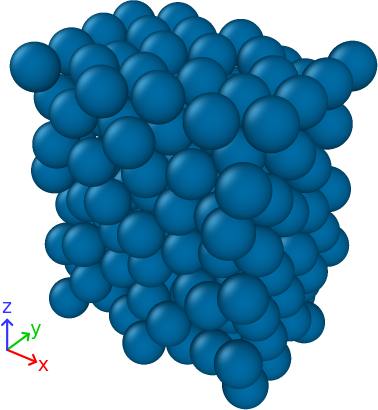
\includegraphics[width = \textwidth]{figures/lbm/lbm-thesis-filled.png}
        \caption{Representative pebble bed having filled the volume to $\phi = 0.61$ with DEM.}\label{fig:lbm-filled}
    \end{subfigure}
    ~
    \begin{subfigure}[b]{0.44\textwidth}
        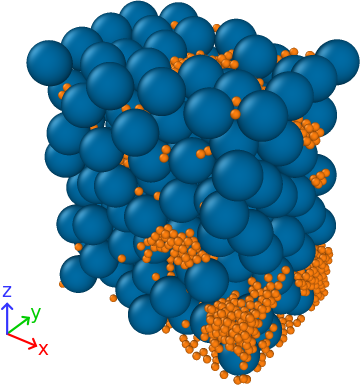
\includegraphics[width = \textwidth]{figures/lbm/lbm-thesis-crushed.png}
        \caption{Pebble bed with $r^* = 0.2$ and $\eta = 0.05$ constructed with DEM.}\label{fig:lbm-crushed}
    \end{subfigure}
    \caption{DEM pebble beds are generated to provide pictures of packings to be loaded into LBM lattices.}\label{fig:dem-for-lbm}
\end{figure}



\subsection{Results \& Discussion}

After mapping DEM pebbles onto LBM lattices, they are run to thermal steady-state. Pebbles, as realized in LBM, are shown in \Cref{fig:lbm-pebble-temperatures-z,fig:lbm-pebble-temperatures-y,fig:lbm-pebble-temperatures-x}, colored by temperature.

\begin{figure}[!ht]
    \centering
    \begin{subfigure}[b]{0.44\textwidth}
        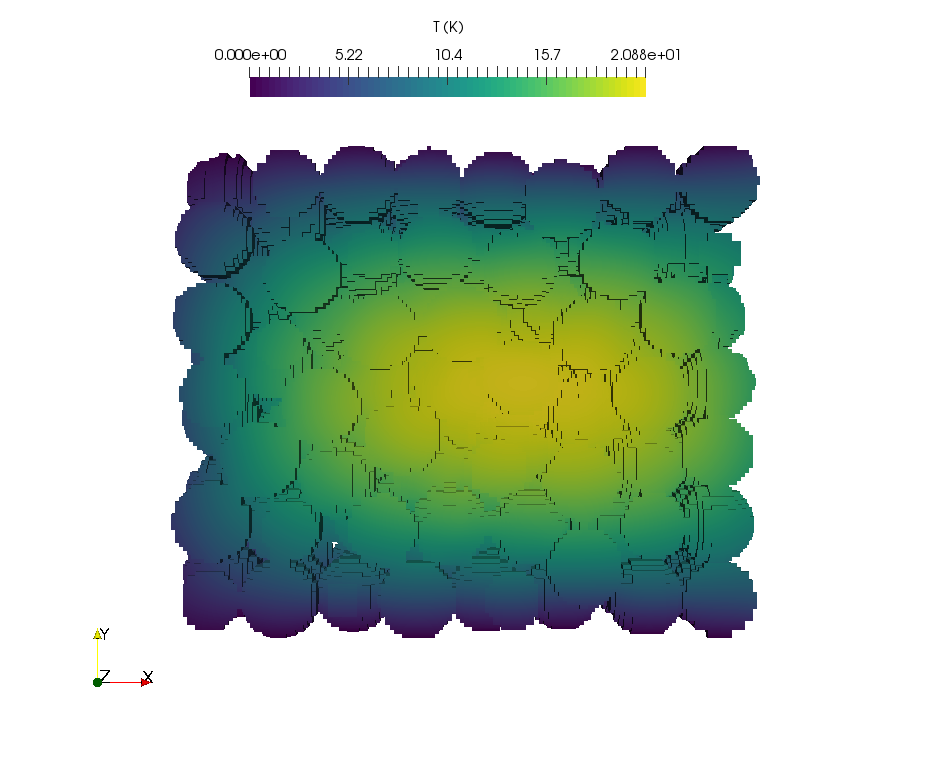
\includegraphics[trim={6cm 6cm 5cm 0cm},clip, width = \textwidth]{figures/lbm/lbm-pebbles-z-normal-filled}
        \caption{Filled}\label{fig:lbm-pebble-temperatures-filled-z}
    \end{subfigure}
    ~
    \begin{subfigure}[b]{0.44\textwidth}
        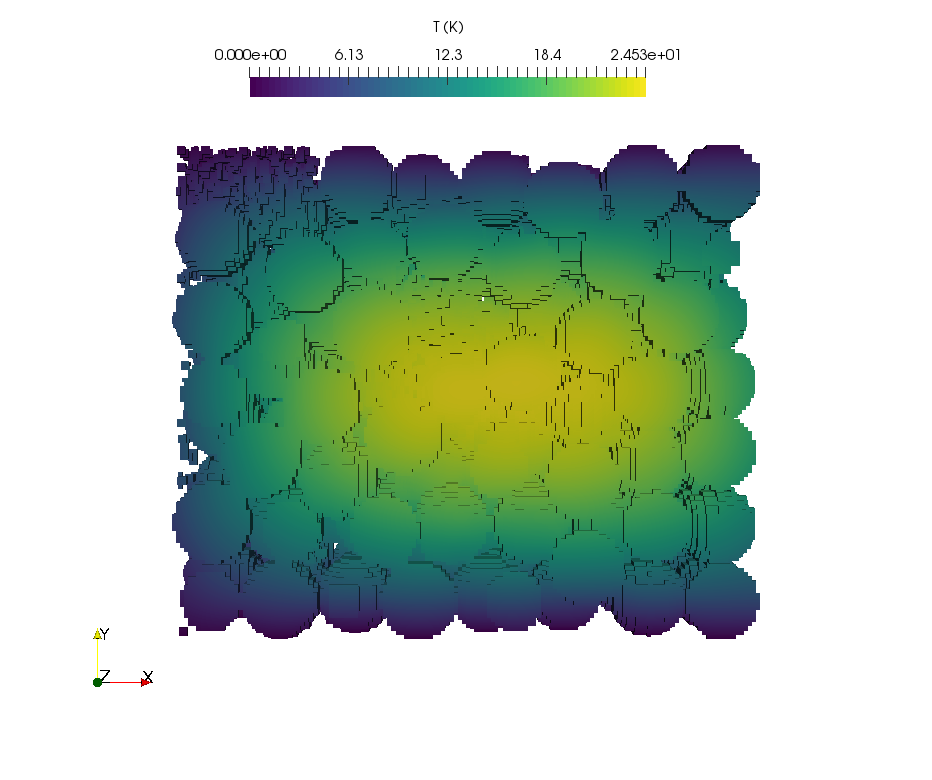
\includegraphics[trim={6cm 6cm 5cm 0cm},clip, width = \textwidth]{figures/lbm/lbm-pebbles-z-normal-crushed}
        \caption{Crushed}\label{fig:lbm-pebble-temperatures-crushed-z}
    \end{subfigure}
    \caption{Frontal view of pebbles realized in LBM lattices (y-normal, fluid moving left to right).}\label{fig:lbm-pebble-temperatures-z}
\end{figure}

\begin{figure}[!ht]
    \centering
    \begin{subfigure}[b]{0.44\textwidth}
        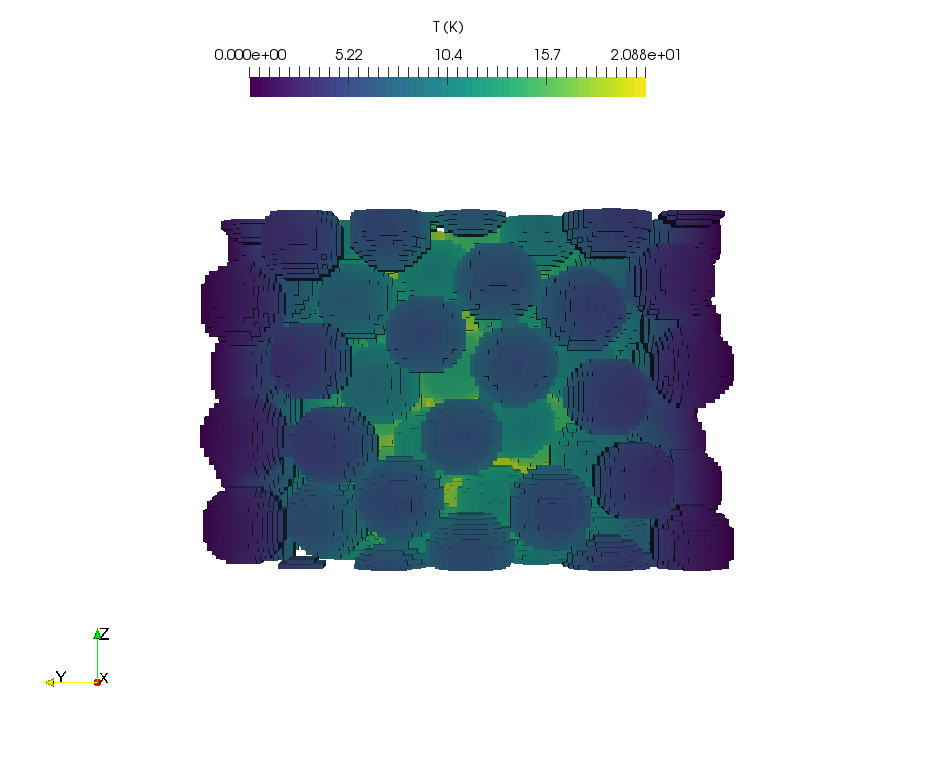
\includegraphics[trim={6cm 6cm 5cm 0cm},clip, width = \textwidth]{figures/lbm/lbm-pebbles-x-normal-filled}
        \caption{Filled}\label{fig:lbm-pebble-temperatures-filled-x}
    \end{subfigure}
    ~
    \begin{subfigure}[b]{0.44\textwidth}
        \includegraphics[trim={6cm 6cm 5cm 0cm},clip, width = \textwidth]{figures/lbm/lbm-pebbles-x-normal-crushed}
        \caption{Crushed}\label{fig:lbm-pebble-temperatures-crushed-x}
    \end{subfigure}
    \caption{Bottom view of pebbles realized in LBM lattices (z-normal, fluid moving into page).}\label{fig:lbm-pebble-temperatures-x}
\end{figure}

\begin{figure}[!ht]
    \centering
    \begin{subfigure}[b]{0.44\textwidth}
        \includegraphics[trim={6cm 6cm 5cm 0cm},clip,width = \textwidth]{figures/lbm/lbm-pebbles-y-normal-filled}
        \caption{Filled}\label{fig:lbm-pebble-temperatures-filled-y}
    \end{subfigure}
    ~
    \begin{subfigure}[b]{0.44\textwidth}
        \includegraphics[trim={6cm 6cm 5cm 0cm},clip, width = \textwidth]{figures/lbm/lbm-pebbles-y-normal-crushed}
        \caption{Crushed}\label{fig:lbm-pebble-temperatures-crushed-y}
    \end{subfigure}
    \caption{Side view of pebbles realized in LBM lattices (x-normal, fluid moving left to right).}\label{fig:lbm-pebble-temperatures-y}
\end{figure}
\FloatBarrier

Streamlines from LBM results are given in \Cref{fig:streamlines-z,fig:streamlines-x,fig:streamlines-y}. In the pebble bed with crushed fragments, the helium flow is clearly more tortuous than the pebbled bed with solid, well-packed pebbles.
\begin{figure}[!ht]
    \centering
    \begin{subfigure}[b]{0.44\textwidth}
        \includegraphics[width = \textwidth]{figures/lbm/temperature-streamlines-filled-z-normal}
        \caption{Filled}\label{fig:streamlines-filled-z}
    \end{subfigure}
    ~
    \begin{subfigure}[b]{0.44\textwidth}
        \includegraphics[width = \textwidth]{figures/lbm/temperature-streamlines-crushed-z-normal}
        \caption{Crushed}\label{fig:streamlines-crushed-z}
    \end{subfigure}
    \caption{Top view of streamlines generated along in a line parallel to $x$-axis (fluid moving left to right).}\label{fig:streamlines-z}
\end{figure}

\begin{figure}[!ht]
    \centering
    \begin{subfigure}[b]{0.44\textwidth}
        \includegraphics[width = \textwidth]{figures/lbm/temperature-streamlines-filled-x-normal}
        \caption{Filled}\label{fig:streamlines-filled-x}
    \end{subfigure}
    ~
    \begin{subfigure}[b]{0.44\textwidth}
        \includegraphics[width = \textwidth]{figures/lbm/temperature-streamlines-crushed-x-normal}
        \caption{Crushed}\label{fig:streamlines-crushed-x}
    \end{subfigure}
    \caption{Rear view of streamlines generated along in a line parallel to $x$-axis (fluid moving into page).}\label{fig:streamlines-x}
\end{figure}

\begin{figure}[!ht]
    \centering
    \begin{subfigure}[b]{0.44\textwidth}
        \includegraphics[width = \textwidth]{figures/lbm/temperature-streamlines-filled-y-normal}
        \caption{Filled}\label{fig:streamlines-filled-y}
    \end{subfigure}
    ~
    \begin{subfigure}[b]{0.44\textwidth}
        \includegraphics[width = \textwidth]{figures/lbm/temperature-streamlines-crushed-y-normal}
        \caption{Crushed}\label{fig:streamlines-crushed-y}
    \end{subfigure}
    \caption{Side view of streamlines generated along in a line parallel to $x$-axis (fluid moving left to right).}\label{fig:streamlines-y}
\end{figure}
\FloatBarrier

A quantitative description of the extra paths taken by fluid packets moving through the crushed pebble bed is tortuosity. Tortuosity was first introduced to studies of porous media by PC Carman in 1937.\cite{Carman1997} Tortuosity is described as the ratio between the effective length of travel of a packet of fluid through a packed bed against the characteristic length of the packed bed (the length the packet would travel in unimpeded flow),
\begin{equation}
\mathscr{T} = \frac{L_\text{eff}}{L}
\end{equation}

Matyka \& Koza provide a method for calculating tortuosity from readily available numerical data.\cite{Matyka2011} Their formula reads,
\begin{equation}\label{eq:tortuosity}
\mathscr{T} = \frac{\langle u \rangle}{\langle u_x \rangle}
\end{equation}

where $\langle u \rangle$ is the average magnitude of the intrinsic velocity over the entire system volume. And $\langle u_x \rangle$ is the average of the component of velocity along the macroscopic flow direction.

Taking advantage of the regularly spaced lattices in LBM, tortuosity can then be calculated directly from LBM results along all nodes,
\begin{equation}
\mathscr{T} = \frac{\sum_{\vec{r}}u(\vec{r})}{\sum_{\vec{r}} u_x(\vec{r})}
\end{equation}

Tortuosity is found for the filled pebble bed to be $\mathscr{T} = 1.245$; for crushed pebble bed it is calculated to be $\mathscr{T} = 1.329$. The crushed pebble fragments caused an increase of 6.7\% to tortuosity of fluid flow.

In \Cref{fig:lbm-contours-40-80,fig:lbm-contours-100-140}, many contours of velocity, normalized against the inlet magnitude, are shown for the filled and crushed pebble beds ($\vec{u}/U_0$). Redistribution of particles from fragmentation result in clogging certain regions and thus localized increases in velocity, compared to the well-packed pebble bed. The velocity jets manifest in regional averages in the pebble bed as well. The results of LBM are integrated along $z$ and $y$ to provide profiles along the direction of interest. Velocity profiles and void fraction are given in \Cref{fig:y-phi-v-profiles} for the cases of well-packed and crushed pebble beds.

\begin{figure}[!ht]
    \centering
    \begin{subfigure}[b]{0.44\textwidth}
        \includegraphics[width = \textwidth]{figures/lbm/cross-sections-filled/contour-40}
        \caption{Filled, height of $2d_p$}\label{fig:lbm-contours-filled-40}
    \end{subfigure}
    ~
    \begin{subfigure}[b]{0.44\textwidth}
        \includegraphics[width = \textwidth]{figures/lbm/cross-sections-crushed/contour-40}
        \caption{Crushed, height of $2d_p$}\label{fig:lbm-contours-crushed-40}
    \end{subfigure}

    \begin{subfigure}[b]{0.44\textwidth}
        \includegraphics[width = \textwidth]{figures/lbm/cross-sections-filled/contour-60}
        \caption{Filled, height of $3d_p$}\label{fig:lbm-contours-filled-60}
    \end{subfigure}
    ~
    \begin{subfigure}[b]{0.44\textwidth}
        \includegraphics[width = \textwidth]{figures/lbm/cross-sections-crushed/contour-60}
        \caption{Crushed, height of $3d_p$}\label{fig:lbm-contours-crushed-60}
    \end{subfigure}

    \begin{subfigure}[b]{0.44\textwidth}
        \includegraphics[width = \textwidth]{figures/lbm/cross-sections-filled/contour-80}
        \caption{Filled, height of $4d_p$}\label{fig:lbm-contours-filled-80}
    \end{subfigure}
    ~
    \begin{subfigure}[b]{0.44\textwidth}
        \includegraphics[width = \textwidth]{figures/lbm/cross-sections-crushed/contour-80}
        \caption{Crushed, height of $4d_p$}\label{fig:lbm-contours-crushed-80}
    \end{subfigure}
    \caption{$x$-$y$-plane contours from heights of $2d_p$ to $4_dp$ show localized peaks of velocity in crushed pebble beds.}\label{fig:lbm-contours-40-80}
\end{figure}



\begin{figure}[!ht]
    \centering
    \begin{subfigure}[b]{0.44\textwidth}
        \includegraphics[width = \textwidth]{figures/lbm/cross-sections-filled/contour-100}
        \caption{Filled, height of $5d_p$}\label{fig:lbm-contours-filled-100}
    \end{subfigure}
    ~
    \begin{subfigure}[b]{0.44\textwidth}
        \includegraphics[width = \textwidth]{figures/lbm/cross-sections-crushed/contour-100}
        \caption{Crushed, height of $5d_p$}\label{fig:lbm-contours-crushed-100}
    \end{subfigure}

    \begin{subfigure}[b]{0.44\textwidth}
        \includegraphics[width = \textwidth]{figures/lbm/cross-sections-filled/contour-120}
        \caption{Filled, height of $6d_p$}\label{fig:lbm-contours-filled-120}
    \end{subfigure}
    ~
    \begin{subfigure}[b]{0.44\textwidth}
        \includegraphics[width = \textwidth]{figures/lbm/cross-sections-crushed/contour-120}
        \caption{Crushed, height of $6d_p$}\label{fig:lbm-contours-crushed-120}
    \end{subfigure}

    \begin{subfigure}[b]{0.44\textwidth}
        \includegraphics[width = \textwidth]{figures/lbm/cross-sections-filled/contour-140}
        \caption{Filled, height of $7d_p$}\label{fig:lbm-contours-filled-140}
    \end{subfigure}
    ~
    \begin{subfigure}[b]{0.44\textwidth}
        \includegraphics[width = \textwidth]{figures/lbm/cross-sections-crushed/contour-140}
        \caption{Crushed, height of $7d_p$}\label{fig:lbm-contours-crushed-140}
    \end{subfigure}
    \caption{$x$-$y$-plane contours from heights of $5d_p$ to $7_dp$ show localized peaks of velocity in crushed pebble beds.}\label{fig:lbm-contours-100-140}
\end{figure}


\begin{figure}[!ht]
    \centering
    \begin{subfigure}[b]{0.44\textwidth}
        \includegraphics[width = \textwidth]{figures/lbm/y-phi-v-profiles-filled.png}
        \caption{Filled}\label{fig:y-phi-v-profiles-filled}
    \end{subfigure}
    ~
    \begin{subfigure}[b]{0.44\textwidth}
        \includegraphics[width = \textwidth]{figures/lbm/y-phi-v-profiles-crushed.png}
        \caption{Crushed}\label{fig:y-phi-v-profiles-crushed}
    \end{subfigure}
    \caption{$y$-$z$-plane averages of normalized velocity (left) and packing fraction (right) demonstrating the oscillatory behavior of flow from ordered packing forced by physical boundaries.}\label{fig:y-phi-v-profiles}
\end{figure}


In \Cref{fig:lbm-cfd-dem-velocity}, velocity profiles as calculated with LBM and CFD-DEM models are given. Comparisons of packing fraction calculated with the two modeling approaches are similarly given in \Cref{fig:lbm-cfd-dem-phi}.
\begin{figure}[!ht]
    \centering
    \begin{subfigure}[b]{0.44\textwidth}
        \includegraphics[width = \textwidth]{figures/lbm/y-v-profiles-filled-cfd-dem}
        \caption{Filled}\label{fig:lbm-cfd-dem-velocity-filled}
    \end{subfigure}
    ~
    \begin{subfigure}[b]{0.44\textwidth}
        \includegraphics[width = \textwidth]{figures/lbm/y-v-profiles-crushed-cfd-dem}
        \caption{Crushed}\label{fig:lbm-cfd-dem-velocity-crushed}
    \end{subfigure}
    \caption{$y$-$z$-plane averages of normalized velocity for LBM (dashed) and CFD-DEM (solid).}\label{fig:lbm-cfd-dem-velocity}
\end{figure}

\begin{figure}[!ht]
    \centering
    \begin{subfigure}[b]{0.44\textwidth}
        \includegraphics[width = \textwidth]{figures/lbm/y-phi-profiles-filled-cfd-dem}
        \caption{Filled}\label{fig:lbm-cfd-dem-phi-filled}
    \end{subfigure}
    ~
    \begin{subfigure}[b]{0.44\textwidth}
        \includegraphics[width = \textwidth]{figures/lbm/y-phi-profiles-crushed-cfd-dem}
        \caption{Crushed}\label{fig:lbm-cfd-dem-phi-crushed}
    \end{subfigure}
    \caption{$y$-$z$-plane averages of normalized packing fraction for LBM (dashed) and CFD-DEM (solid).}\label{fig:lbm-cfd-dem-phi}
\end{figure}









% DIspersion section ~~~~~~~~~~~~~~~~~~~~~~~~~~~~~~~~~~~~~~~~~~~~~~~~~~~~~~~~~~~~~~~~~~~~~~~~~~~~~~~~~~~
Thermal dispersion is the spreading of heat caused by variations in velocity about a mean in a fluid. In a packed bed with stagnant interstitial fluid, molecular thermal diffusion is the dominant mode of heat transfer. Mechanical dispersion of heat and fluid flow becomes significant with increased Reynolds number in pores, leading to additional heat transfer. We will quantify thermal dispersion with a commonly-applied temperature-gradient assumption to calculated a dispersion conductivity.\cite{Kuwahara1996,Nakayama2006,Yang2010a}

Applying volume-averaging-theory (VAT), the intrinsic energy equation for a fluid in porous media in a representative elemental volume (REV) is given in Sbutega\etal\cite{Sbutega2013},
\begin{equation}
\epsilon\rho_fC_{pf}\langle\vec{u}\rangle^f\cdot\nabla\langle T_f\rangle^f = \nabla\left(\vec{k}_{f,\text{eff}}\cdot\nabla\langle T_f\rangle^f \right) + hS_w\left(\langle T_s\rangle^s - \langle T_f\rangle^f\right)
\end{equation}
where $\langle T_f\rangle^f$ is the intrinsic volume average of fluid temperature and $\langle T_s\rangle^s$ is the intrinsic volume average of solid phase temperature. $h$ is a closure term for heat transfer coefficient between solid and fluid phases which is applied over the volumetric interfacial surface area, $S_w = A_{fs}/V$, in the REV. The effective conductivity for the fluid is a tensor that is composed of the stagnant thermal conductivity, including diffusive conductivity and the `tortuousity' conductivty, and the dispersion conductivity,
\begin{equation}
\vec{k}_{f,\text{eff}} \cdot\nabla\langle T_f\rangle^f  = \vec{k}_{i,\text{stag}}\cdot\nabla\langle T_f\rangle^f + \vec{k}_{i,\text{disp}}\cdot\nabla\langle T_f\rangle^f 
\end{equation}
where
\begin{align}
\vec{k}_{f,\text{stag}}\cdot\nabla\langle T_f\rangle^f &= \epsilon k_f \nabla\langle T_f\rangle^f + \frac{1}{V}\int_{Afs}\! T_f \,\mathrm{d}\vec{A} \\
\vec{k}_{f,\text{disp}} \cdot \nabla \langle T\rangle^f &= -\epsilon\rho_f C_{pf}\langle T_f' \vec{u}_f'\rangle^f
\end{align}

Sbutega\etal~and Kuwahara\etal\cite{Sbutega2013,Kuwahara2001} show that the dispersion conductivity is negligible at low Peclet number but dominates at high Peclet. In the pebble beds of solid breeders, low Peclet numbers are expected due to slow moving purge gas and small Prandtl number of helium. As a consequence, we can expect that temperatures calculated \textit{via} the lattice-Boltzmann method should not be fundamentally different from CFD-DEM computations. Nevertheless, data of the LBM model allow us to calculate dispersion conductivities; for the well-packed bed we find the average of the $y$-component of dispersive conductivity to be only $k_{f,\text{disp}}|_y =\SI{0.0043}{\watt\per\meter\per\kelvin}$; for the bed with crushed pebbles the $y$-componenet of dispersive conductivity is $k_{f,\text{disp}}|_y =\SI{0.0053}{\watt\per\meter\per\kelvin}$; an increase of 23.2\% for crushed pebbles. Nevertheless, in both cases the amount of spreading due to dispersive conductivity is negligibly small. Therefore, in the beds we have analyzed with small Peclet number, the results of CFD-DEM and LBM are predictably similar. Temperature profiles, averaged in slices of $y$- and $z$-directions, calculated from LBM and CFD-DEM for well-packed and crushed beds are given together in \Cref{fig:lbm-cfd-dem-temperatures}.

\begin{figure}[!t]
    \centering
    \includegraphics[width = 0.75\textwidth]{figures/lbm/cfd-lbm-T-profiles}
    \caption{Temperature profiles in pebble beds that are fully filled (solid), and with 5\% crushed (dashed) using both CFD-DEM (blue) and LBM (orange) models.}\label{fig:lbm-cfd-dem-temperatures}
\end{figure}

In \Cref{fig:lbm-cfd-dem-temperatures}, we see extremely good agreement between CFD-DEM and LBM results, particularly for well-packed pebble beds.. While the velocity profiles between the two methods showed only qualitative similiarties, the lack of mechanical dispersion of heat from the $\langle T_f' \vec{u}_f'\rangle^f$ term allows the volume-averaged approach of CFD-DEM to model heat transfer as faithfully as LBM. In pebble beds with fragmentation, the agreement between CFD-DEM and LBM is less. The temperatures from LBM are 6\% higher at the midpoint. Lower temperatures in LBM are, in part, not physical but attributable to the resolution when mapping DEM pebbles into LBM. A resolution of 20 pixels was chosen to represent pebbles. Fragments of size $r^* = 0.2$ result in 4 pixels per diameter for fragments. As an example, a slice of pebble bed (pebbles in black, fluid in white) is shown in \Cref{fig:lbm-fragment-contact-area}. In this cross-section, the small fragments mapped into LBM have larger contact areas than Hertzian predictions provide in DEM. 

\begin{figure}[!t]
    \centering
    \includegraphics[width = 0.65\textwidth]{figures/lbm/fragment-contact-resolution}
    \caption{Over-estimates of contact area of fragments contributes to higher heat conductance in LBM model than CFD-DEM.}\label{fig:lbm-fragment-contact-area}
\end{figure}






\FloatBarrier

\subsection{Conclusions}
Much effort was made to accurately model the tortuous flow of helium in packed beds. Using the lattice-Boltzmann method, we looked into pore-scale influences of crushing on void fraction distribution and consequently velocity fields of pebble beds. We found that when 5\% of pebbles are fragmented, tortuosity of the pebble bed increased by nearly 7\% while the dispersive conductivity increased over 23\%. In spite of the increase in dispersive conductivity, the impact on temperature profile spreading remained negligibly small due to the low Peclet number flow expected in tritium breeding blankets. The result, however, does inspire a path of research toward allowing higher power density in solid breeders. The pebble bed with crush fragments studied here can be considered as a low-porosity, polydisperse pebble bed. Polydispersity in pebble beds can lead to very high packing fractions.

Yang \& Nakayama provide a correlation for transverse dispersive conductivity in regularized packings as a function of a modified Peclet number,\cite{Yang2010a}
\begin{equation}
\frac{k_\text{diss}}{k_f} = 0.0075 \frac{\Pe_D^2}{2+1.1\frac{\Pe_D^{0.6}}{\Pr^{0.27}}}
\end{equation}
where the Peclet number,
\begin{equation}
\Pe_D = \rho_fC_{pf}\frac{\langle u \rangle d_p}{k_f}
\end{equation}
is based on the Darcian velocity, $\langle u \rangle = \frac{U_0}{\epsilon}$. Because the Darcian velocity increases with more tightly packed beds (smaller void fraction), there appears to be some control over dispersive conductivity by means of polydisperse packings. Using material properties for helium and \SI{1}{\milli\meter} pebbles (neglecting for a moment the influence of polydispersity), we can calculate dispersive conductivity as a function of void fraction. In \Cref{fig:lbm-dis-peclet}, the example calculation is shown as a function of packing fraction. Experimentally, packing fractions in polydisperse beds can easily reach $\phi = 0.80$.\cite{Reimann:2000tw} From \Cref{fig:lbm-dis-peclet}, dispersive conductivity (again, calculated assuming single sized pebbles) increases by an order of magnitude for packing fractions around $\phi =0.88$.

\begin{figure}[!t]
    \centering
    \includegraphics[width = 0.65\textwidth]{figures/lbm/peclet-dispersive-conductivity}
    \caption{Dispersive conductivity for pebble beds increases rapidly as packing fraction approaches unity.}\label{fig:lbm-dis-peclet}
\end{figure}

Large packing fractions are generally avoided in solid breeder blankets in order to avoid their concomitant increase in pressure drop. However, from the investigation performed with heat transfer in lattice-Boltzmann simulations, it is worth revisiting the topic from the point of view of energy management and the ability for packed beds to sustain larger power densities.

The lattice-Boltzmann method allowed us to study the tortuous path of helium through packed beds of spheres with and without crush fragments. Unlike traditional CFD methods for packed beds, no simplifications of contact regions was required and a direct mapping, which maintained consistency of packing fractions, was performed when digitizing DEM packing structures onto LBM lattice nodes. LBM simulations were run on a machine with quad-core, 3 GHz Intel Xeon E6-1607. Computation times for the lattices with a resolution of 20 voxels per diameter, up to 400 seconds of real time simulation were generally around 30 hours. On the same machine, CFD-DEM simulations generally concluded in approximately 4 hours. Scaling up to a full-size pebble bed would require significant computational expenses. Yet, owing to the small Peclet number of pebble beds under consideration, there does not appear to be any evidence that considerations of the entire helium flow field is necessary when attempting to model thermomechanical interactions of solid breeders. The lattice-Boltzmann technique can, however, help in studying novel concepts for increasing heat transfer in packed beds in order to increase power density, such as the increase in dispersive conductivity due to mixed pebble beds and high packing fractions.